%\documentclass[twoside,openright]{uva-bachelor-thesis}
\documentclass[twoside,openright,notitlepage]{uva-bachelor-thesis}

%\usepackage[dutch]{babel}  % uncomment if you write in dutch
\usepackage{graphicx}
\usepackage{url}
\usepackage{setspace}
\usepackage[export]{adjustbox}[2011/08/13]
\usepackage{placeins}
\usepackage[toc,page]{appendix}
\usepackage[backend=bibtex,
style=numeric
%style=alphabetic
%style=reading
]{biblatex}
\addbibresource{references}

\renewcommand{\baselinestretch}{1.2} 

% Title Page
\title{Trusting websites using geographical consistency}
\author{Laurens Verspeek}
\supervisors{Raphael `kena' Poss (UvA)}
\signedby{Raphael `kena' Poss (UvA)}

\begin{document}
\maketitle

\begin{abstract}
With the growth of the Internet and its increasingly important role in our lives, there is also an increase in the number of malicious websites on the web. There are already several techniques to detect malicious websites, but none of these techniques take the geographical features of the different technological components of a website into account. These features can be used to determine the geographical consistency of a site, which might help the user with correctly classifying websites. First, different technological components of a website that may have a location are examined and different methods are researched to retrieve the geographical locations of these components. Then the strategies for the presentation of the retrieved information and good ways to combine that information are explained and discussed. This knowledge results in an API and a tool for the user which might help the user classify websites. An experiment where the participants had to classify websites with and without the tool shows that the tool in its current form improves the classification of both malicious and normal websites significally and also improved the certainty of the classifications. This proves that geographical consistency is a relevant way to determine the trustworthiness of websites.
\end{abstract}

\tableofcontents

\chapter{Introduction}
While the internet has become an essential part in our daily life, the growth of the web has also created a platform for supporting a wide range of criminal activities such as spam, phishing or malware. A factor common to most malicious web sites is the use of different geographical regions for different technologies and components of the website. The domain name is registered in one country, the SSL certificate in another, the IP address of the server perhaps in yet another. There are quite a few other components which can have a different geographical location. For example, the user browsing from the malicious web site to a payment engine will often also cross a country boundary. This geographical separation is highly unusual in "honest" web sites. Many such dishonest activities could thus be detected (and prevented) by geolocating the different technological components involved in the trust relationship between user, browser, web server and web site.
\section{Research questions}
There are many other features of a website, such as the page content or the lexical features of the Uniform Resource Locator (URL), which might play a role in classifying a website as trustful or malicious. A lot of research has been done to develop tools and techniques to detect and study the presence of threats on the web. However, these studies almost never take the geographical locations of different components of a website into account and if they do, it is on a very basic level. This thesis focusses on geographical consistency of different components of a website and how this relates to malicious websites and other features of a website as mentioned before will be left out of consideration for the time being. Thus the main focus in this thesis is the geographical consistency of websites and therefore the main question and the motivation for this thesis is:\\\\
\emph{How can geographical locations from different components of a website help the user to evaluate the trustworthiness of a website?}\\

Answering this question requires extensive research, so we propose to initiate this work by first focusing on four prerequisite questions formulated as follows:
\begin{enumerate}
  \item \emph{Which technological components with a location might play a role in trusting a website?}
  \item \emph{How to find the geographical location of these different components?}
  \item \emph{How to combine and visualize this information about geographical location in order to say something about the trustworthiness of websites?}
  \item \emph{How to implement the back and front-end for the visualization of this information?}
\end{enumerate}

\section{Related work}
Previous studies about detecting malicious websites mainly focused on the (lexical) features of the domain name of a website. Research of Ma, Justin, et al.~\cite{ma2009beyond} showed that by looking at lexical properties of website URLs, a lot of malicious websites can be detected. The automatic classification of the URLs as either malicious or benign is based on supervised learning across both lexical and host-based features. However, the only geographical-based property this research took into account was the geographical location of the host itself. \\

Research of Cherukuri, Manoj, and Srinivas Mukkamala~\cite{cherukuri2011link} visualized the geographical locations of malicious websites and showed the fact that the malicious websites are not limiting the hosting to a country or a hosting service but are spread all over. So the geographical property of the host on its own contributes very little to the classification of websites, like in the research of Ma, Justin, et al.~\cite{ma2009beyond} Studies similar to the last mentioned research in terms of features of the website are CANTINA~\cite{zhang2007cantina}, which classifies phishing URLs by looking at a weighted sum of 8 features (4 content-related, 3 lexical, and 1 WHOIS related) and the work by Garera et al.~\cite{garera2007framework}, where logistic regression over 18 hand-selected features is used to classify phishing URLs. McGrath and Gupta~\cite{mcgrath2008behind} perform a comparative analysis of phishing and non-phishing URLs based on features such as WHOIS thin records (containing date and registrar-provided information only), geographical location of the host and lexical features of the URL (length, character distribution, and presence of pre-defined brand names). \\

All of these techniques use URL-based classifications of websites. Provos et al.~\cite{mavrommatis2008all} perform a study of drive-by exploit URLs and use a patented machine learning algorithm as a pre-filter for VM-based analysis. Unlike the previous approaches, they extract content-based features from the page. Prophiler, a research of Canali, Davide, et al.~\cite{canali2011prophiler}, uses a set of models that evaluate the features extracted from the content of a website. These two studies provide content-based classification of website. The latter one even looks at both URL-based features and content-based features of websites, but the only geographical feature is the location of the first IP address returned.

\section{Contribution}
As stated above, all of the previously mentioned research use no or very little geographical features in their classification of websites. However, there are lot of technological components of a website with a geographical location which might play a role in detecting malicious website. The location of the various components individually contributes very little to the classification of a website, but the relation of the location of the components can be a very powerful combination in order to say something about trusting websites.\\

The answers to the four prerequisite sub questions stated in the \emph{Research questions} section will already enable the user to classify a website as trustful or malicious. However, automatically detecting and preventing dishonest activities of malicious websites by looking at the different geographical locations requires extensive research on the relation of the locations and malicious websites. Based on the research questions, this thesis will lay the foundation for this research. With the knowledge gained from this research an implementation and visualization of the solution to the 'trusting websites problem' based on the results of this thesis is proposed and evaluated.

\chapter{Background}

\section{Existing security techniques}
\subsection{Static and dynamic analysis}
Current research about detecting malicious websites and existing approaches can be categorized into two complementary analysis methods: static and dynamic analysis. Static analysis focusses mainly on static features such as the web page content (or the source code), the domain name structure, host-based information etc. to find the characteristics of malicious websites. Dynamic analysis is more focused on capturing behaviors which occur when the page is loaded in a controlled environment.~\cite{eshete2011malicious} Both these different types of analyses extract features of some type. These features are used for the classification of malicious websites. The algorithm to classify the websites is often trained using machine learning techniques. A few techniques which use this sort of analysis are discussed in the \emph{Related work} section.

\subsection{Honey-clients}
Client Honeypots are active security devices that mimic a human visitor to search malicious servers that attack clients. The honey-client acts as a client and when a website is being rendered, the behavior is captured and analyzed. There are three types of classification for honey-clients. This classification is based on their interaction level, which can be high or low. This interaction level denotes the level of functional interaction the server can utilize on the client honeypot. 

\subsubsection{High-interaction}
High-interaction honey-clients, such as \emph{HoneyMonkey}~\cite{wang2006automated}, have no functional limitations and are comparable to real systems with real clients. Attacks on high-interaction honey-clients are detected via integrity changes in system states after interaction with a server. 

\subsubsection{Low-interaction}
Low-interaction honey-clients, such as \emph{HoneyC}~\cite{seiferthoneyc} and \emph{Monkey-spider}~\cite{ikinci2008monkey}, use lightweight clients to interact with the server and they do not utilize an entire real system. The responses the honey-client gets from a server are analyzed directly in order to detect if an attack has taken place.\\
Low-interaction honey-clients are faster and more lightweight than high-interaction honey-clients. However, because the attack have to be known to the honey-client, they are more likely to ignore new types of attacks. The simplicity of low-interaction honey-client also makes it easier for a malicious website to detect the presence of the honey-client.

\subsubsection{Hybrid honey-clients}
The last classification, hybrid honey-clients, is based on newly hybrid approaches which combine the usage of both high and low interaction detection techniques.\\

Honey-clients, especially high-interaction ones, can give deep insight in the sort of attacks used in malicious website.
The problem is that they need to load and execute each page in order to do their analysis and this can be very resource intensive. Another problem is that not all malicious websites are launching their attack when the website gets visited. Some need user interaction to deploy their attack or use a time-bombs before launching their attack. Honey clients may have a hard time in order to detect such malicious websites. As honey clients are usually a source for blacklists of malicious websites (see next section), the malicious websites are also likely to maintain a blacklist of IP-addresses of honey-clients. Honey-clients can for example be detected through advanced fingerprint identification techniques or simple CAPTCHA verifications, which necessarily needs human interaction.~\cite{qassrawi2011detecting}

\subsection{Blacklisting}
Blacklisting of known malicious websites is a widely used protection technique~\cite{malwareblacklist,phishtank,wot}. These malicious websites are collected via manual reporting, honeypots, and analysis techniques, such as the ones discussed in the previous sections. The advantage of blacklisting is that it is lightweight to deploy and easy to use. However, blacklisting is only useful if they exhaustively identify malicious websites and get updated frequently. \\

In practice, doing this is infeasible due to the fact that new malicious websites arise too often and too fast to be able to blacklist them and due to the fact that malicious sites can be evaluated incorrectly (e.g., due to "cloaking")~\cite{ma2009beyond}. Also, owners of malicious websites often frequently change where the sites are hosted.  

\section{Technological components of websites}
Given the common and specific limitations of \emph{Related work} and \emph{Existing security techniques} as pointed out in these sections, an effective analysis method for detecting malicious websites needs to be found. The basis for an effective analysis is a set of features which are pertinent to the fast-changing malicious websites. As stated earlier in the \emph{Related work} section, analysis methods which look at URL-based features or content-based features of websites or even both have shown some good results in detecting malicious websites. However, the feature-set of these analyses always lack the presence of geographical features of websites. There are many components of the website browsing process which can have a geographical location. Especially the relation between these geographical locations can be very useful in the detection of malicious websites. In order to find these locations, the first thing needed is to know \emph{which technological components with a location might play a role in trusting a website.}

\begin{figure}[h!]
    \centering
    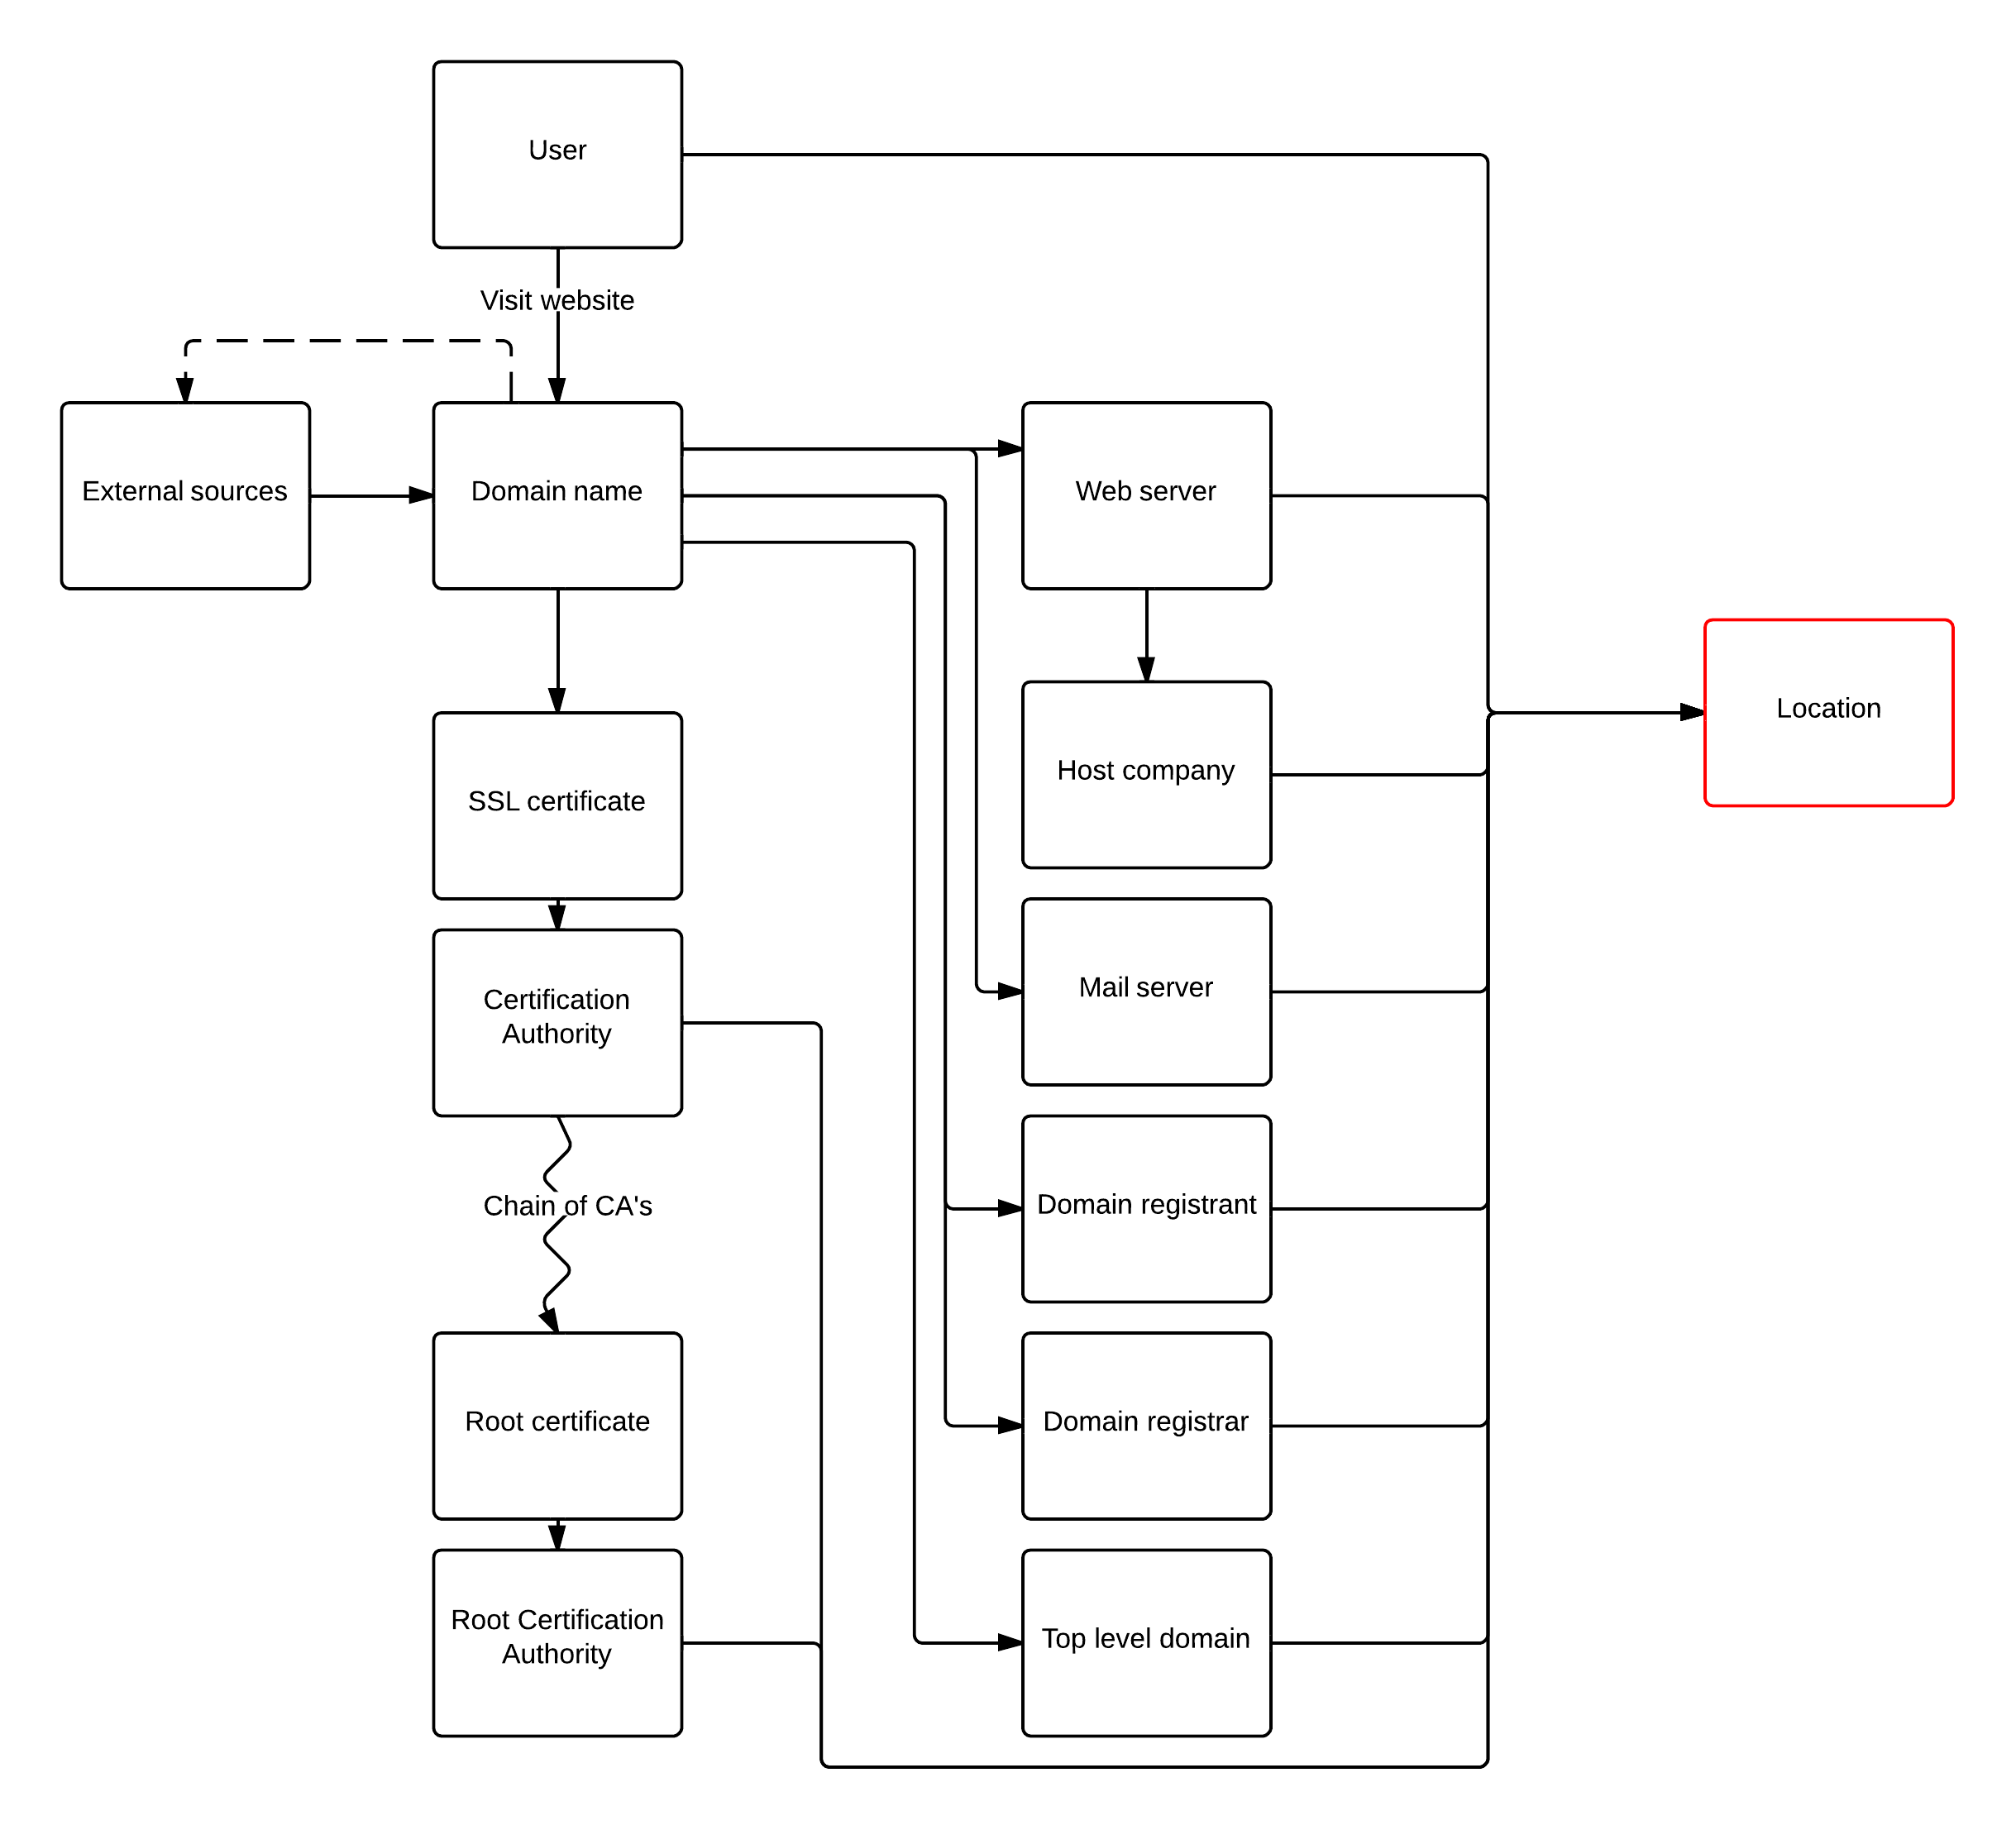
\includegraphics[width=1.2\textwidth, center]{img/components_new_empty.png}
    \caption{Technological components of a website with a location}
    \label{fig:components}
\end{figure}

\subsection{The user}
The web browsing process starts with us, the users. A user is visiting websites with his computer or some other device. Each of these computers and devices that uses the Internet Protocol for communication have an Internet Protocol address (IP address). The users, or actually the devices of these users, all have a physical location which can be used for determining the geographical consistency.

\subsection{Domain name}
A domain name is an identification name in the Domain Name System (DNS).
A domain name represents one or multiple Internet Protocol (IP) resources, such as a server computer hosting a web site. In the fourth quarter of 2013, the number of active domains reached 271 million~\cite{verisign}.\\

Domain names are organized in hierarchical levels in the DNS. As you can see in figure ~\ref{fig:components} the domain name itself does not have a location. However, there are some instances related to domain names which might have a geographical location:

\subsubsection{Top Level Domain}
A top-level domain (TLD) is the first level in the hierarchical DNS. For the domains in lower levels in the hierarchy, the part after the last dot is the TLD. For example, in the domain name "www.uva.nl", the TLD is "nl". Some of the TLD's, like "nl", are linked to a country. For example, "nl" is the TLD for The Netherlands. Some TLD's are not linked to a country, like "com" and "org", but from the others TLD's their geographical features on country-level can be found.

\subsubsection{Domain registrar}
A domain name registrar is a commercial entity or organization that manages and sells the reservation of domain names. The domain registrar might also have a geographical location.

\subsubsection{Domain registrant}
The domain name registrant is the person or company that holds the right to use a specific domain name, which they reserved at a domain registrar.
Like the domain registrar, the domain registrant also has a geographical location.

\subsection{The web server}
As said before, a domain name represents one or multiple Internet Protocol (IP) resources. These resources are the web servers, where the website is hosted. The term web server can refer to either the hardware (the computer) or the software on this hardware. One domain name can have multiple servers. Each of these servers have a physical location.

\subsubsection{Hosts (Server owners)}
Webhosts are companies or commercial entities that provide space on a server owned or leased for use by clients. These companies also have a location.

\subsubsection{Mail server}
Some websites use mail servers. A mail server is a computer that transfers e-mail messages to computers. In the Domain Name System, mail servers are linked to domain names with a mail exchanger (MX) record. Just like a web server, the mail server also has a geographical location.

\subsection{External sources}
Websites often use scripts or data from external sources. It is also quite often the case that data is sent to external sources. For example, the payments in webshops or the login procedures on some sites are often handled by external third-parties. All of these external sources also have a domain name. The domain names of the external sources can be used to recursively get all the geographical locations of components linked to these domain names.

\subsection{SSL Certificates}
An Secure Sockets Layer (SSL) certificate is a digital certificate that authenticates the website's identity and sets up an encrypted connection between the web server and the user's browser using SSL technology. The reason why SSL Certificates are discussed is that these digital certificates get issued by certification authorities.

\subsubsection{Certification authorities}
A certification authority (CA) is a third party that is trusted by both the owner of the certificate and the device of the user visiting the website.\\

In order to validate the trustworthiness of a certification authority, the certification authority has a certificate issued by a certification authority that reside higher in the hierarchy. These types of certification authorities are called intermediate certification authorities. At the top of the hierarchy are the root certification authorities, which sign root certificates. Root certificates are issued by themselves. So in order to establish trust, no further checking of certificates is necessary or possible. This hierarchy of certificates is called \emph{The Chain of Trust}. (see figure ~\ref{fig:cot})\\

\begin{figure}[h!]
    \centering
    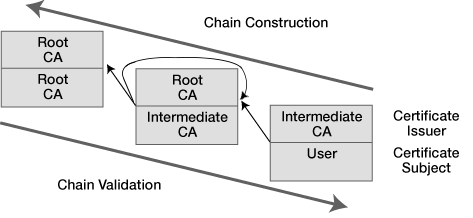
\includegraphics[width=0.7\textwidth]{img/chain_of_trust.png}
    \caption{Chain of Trust}
    \label{fig:cot}
\end{figure}

Each of these certification authorities in the Chain of Trust have a geographical location which may be useful in determining the trustworthiness of a website. This may be useful, because in principle SSL certificates are used to determine trustworthiness, but it is also the case that "bad" CAs exist that certify malicious websites . This can occur by attacking the CA organization, or corruption, or the intervention of a dubious government (for data collection / industrial espionage)~\cite{wsj}. That is why nowadays SSL certificates can no longer serve as sufficient "proof" of trustworthiness.


\FloatBarrier
\chapter{Methods for data collection}
Now that the different technological components of the web browsing process are known, the geographical locations of these components need to be found. In this chapter the various methods of \emph{finding the geographical location of these components} are researched and discussed.

\section{Parsing URL}
In order to find the base domain name, the protocol and the top-level domain of a website, the website's URL needs to be parsed. The domain name can be used for the DNS lookup and for WHOIS (see sections below). The protocol of a website (like HTTP or HTTPS) can be used to determine if a website has SSL certificates. The TLD can be used to determine to which country a websites belongs in case the TLD is a country-specific TLD. To know which TLD belongs to which country, a simple list or database can be used to map the TLD's to their correct country.

\section{Domain Name System lookup}
In order to find more information about the domain name, that domain name can be looked up in the Domain Name System (DNS). The Domain Name System is a hierarchical system that translates names of computers or other resources connected to the Internet to the numerical IP addresses needed for geolocating these resources.\\

Besides the IP-address of the host of the website (A or AAAA record), the DNS also stores other records, such as nameserver records (NS) or mail exchanger records (MX). It also provides CNAME records. CNAME is an abbreviation for Canonical Name. CNAME records are used to specify that the original domain name uses the IP address of another domain name. This domain name is called the canonical domain.~\cite{mockapetris1987domain}\\

The DNS does not provide information about the geolocation
of any of the previously discussed components, but it does give information that can be used to find geolocations.

\section{IP-address to geolocation}
Now that the IP-addresses of the domain name are available (IP-addresses of the hosts, canonical domains and mail servers) and the IP-address of the user, their geolocations need to be found. Geolocation refers to identifying the geographic location of a computer, resource or a user. Geolocation services use a variety of data collection techniques to determine the location of an IP-address.

\subsection{Accuracy of geolocating services}
There are many IP-address to location services available online. The accuracy of these services are often around the 99 percent for country-precision and 60-70 percent for city-precision.~\cite{ipapi,hostapi,ipinfodb,geobytes,ip2loc,maxmind}\\
The accuracy of these services is sufficient for the purpose of this research, since the country-precision is the most important feature that should be accurate.\\

One of these IP-address to geolocation API's~\cite{ipapi} is used in the implementation proposed by this thesis, which is discussed in the \emph{Implementation} chapter.

\section{WHOIS}
WHOIS is a query-response protocol used to lookup information related to IP-addresses or domain names. If a WHOIS-server receives a query it amongst other things returns information about address details of the registrar and registrant of a domain name or address details of the host owner of an IP-address. See the \emph{Technological components of websites} section for more information about the registrar, registrant and host owner. WHOIS is also used for a wider range of information, but for the purpose of finding locations the previously mentioned information is sufficient. The WHOIS protocol delivers the information in a human-readable format.\\

However, due to the inconsistency of the format of the information it is quite difficult to extract the right information for all domain names and IP-addresses automatically. This inconsistency is due to the fact that each country has different laws about which information a WHOIS-server is allowed to return after a query. Even within a country you often see differences in the format of the WHOIS information for domain names or IP addresses. \\

There are a few WHOIS parsers available on the internet, but none of them are good enough to provide the information as mentioned in the previously paragraph. Therefore a WHOIS Parser needs to be implemented which will fetch this information. The implementation of such a parser is discussed in the \emph{Implementation} chapter.

\section{Retrieving SSL certificates}
In order to get the locations of the certification authorities (see section \emph{SSL Certificates} in chapter \emph{Technological components of websites}), the SSL certificates of a website need to be retrieved. These certificates contain the addresses of the certification authorities. By making a request to a website with certain headers that tell the request to verify the website, the ssl certificates are sent as response and the addresses of the certification authorities can be parsed from the certificates. 

\section{Geocoding}
Now that the addresses of all the components are available, they need to be converted into geographic coordinates (latitude and longitude). The geographic coordinates can be used to visualize the position on a map. This converting process is known as Geocoding. An online service that does this converting step is the Google Geocoding API~\cite{google1}. This service also returns the boundaries of the location. This information can be used to determine the precision of the location. See chapter \emph{Strategies for data presentation} for more information about this precision.

\section{Intercepting headers}
When data is received from or sent to external sources. When such data is transmitted, the data is preceded by a header, which contains information such as the sender and the recipient. When a website sends a request to an external source, the header can be examined to find out the domain name of the external source. The chrome webrequest API~\cite{google2} can intercept and read these headers. The implementation of this API can be found in chapter \emph{Implementation}.\\

The domain names of the external sources can again be used to find all location of the different components of these external sources with the same methods as described in the previous sections of this chapter.

\section{Resulting scheme}
With the second sub question answered as well, the scheme in figure \ref{fig:components} with the different technological components can now be extended with the methods to collect these components and their locations. The resulting scheme can be found in figure \ref{fig:components_full}.

\begin{figure}[h!]
    \centering
    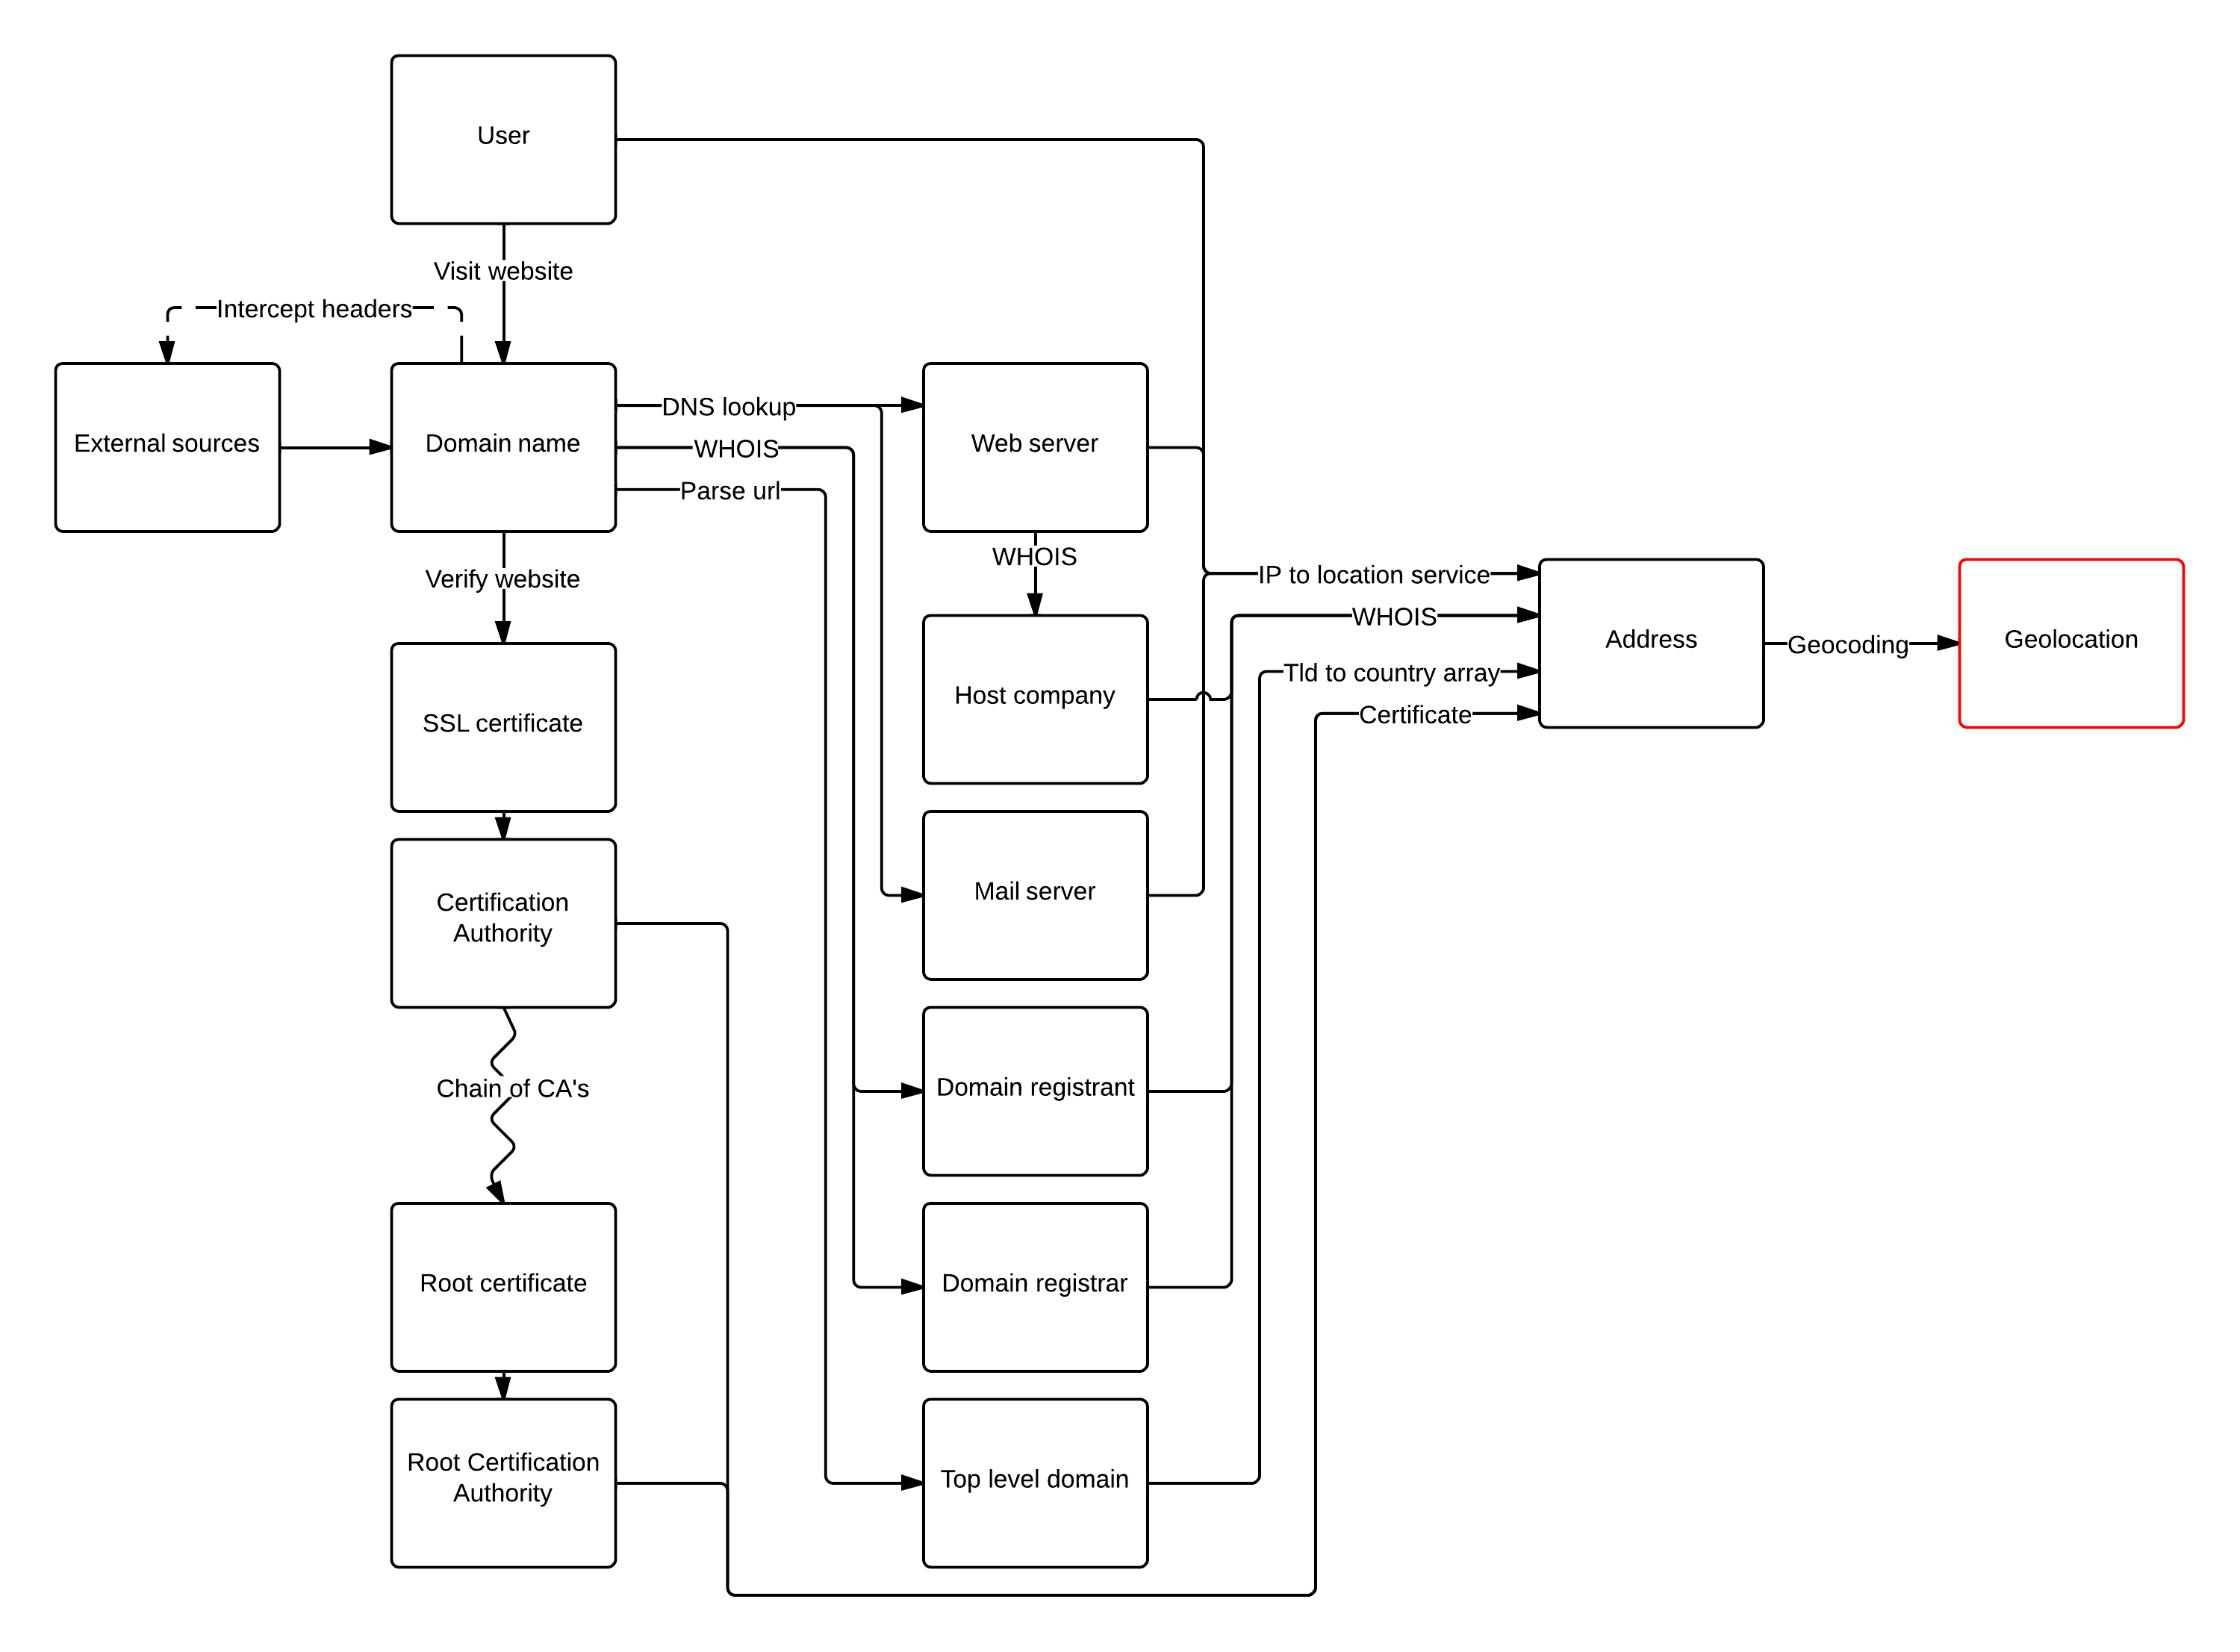
\includegraphics[width=1.3\textwidth,center]{img/components_new.png}%
    \caption{Technological components of a website with a location - complete}
    \label{fig:components_full}
\end{figure}

\FloatBarrier
\chapter{Strategies for data presentation}
Each geographical location of these components on its own will not help much with the classification of websites. However, the geographical consistency of these locations can be very useful in classifying websites. Therefore, \emph{this information needs to be combined and visualized in such a way that the user is able to say something about the trustworthiness of websites.} \\

This chapter will explain and discuss the strategies that can be used to combine and visualize the information about the different locations in a useful way.

\section{Display locations on a world map}
With the geographical locations of the different technological components now available, these locations can be displayed on a world map as points. Such a map would give the user already a good overview of the locations of the components and how they are located relative to each other.\\

For the user to be able to see which points on the map belong to which components, the points should have different colors. Each color represents a component or a set of components. To see more detailed information about each point, the user should be able to click on a point whereupon a popup with text appears with more information about the component the point belongs to.

\section{Directed tree}
To show the connection between the different locations, the locations can be displayed on the map as a directed tree structure. A tree is a hierarchical structure in which any two vertices are connected by exactly one path without cycles. A directed tree is a tree where the paths have one direction. The vertices in the directed tree are the locations on the map and the paths of the tree are the connections between those locations. These connections can also be seen in figure \ref{fig:components_full}, where the arrows between the components are the connections.

\section{Midpoint of weighted locations}
In order to combine the locations and to be able to say something about the geographical consistency, the 'average' location needs to be found. This average can be seen as the midpoint of the website. The algorithm to calculate this midpoint has to take the curvature of the Earth into account. The simple Pythagorean equation is not sufficient to achieve this, since the Pythagorean algorithm only works for flat surfaces. The algorithm also needs to deal with the fact that the locations are not equally important and have different accuracies. \\

The following algorithm finds the center of gravity for the locations of the different components. The longitude and latitude for each location are converted into Cartesian (x,y,z) coordinates. These Cartesian coordinates are then multiplied by the weighting factor of the locations and added together. A line can be drawn from the center of the earth out to this new x, y, z coordinate, and the point where the line intersects the surface of the earth is the geographic midpoint. This surface point is converted into the latitude and longitude for the midpoint.~\cite{midpoint}\\ 

Step by step details of this algorithm: 
\begin{enumerate}
\item Convert the longitude and latitude of a location from degrees to radians:\\
$lat_r = lat \times  \frac{\pi}{180}$\\
$lon_r = lon \times \frac{\pi}{180}$
\item Convert longitude and latitude in radians to Cartesian coordinates (x, y, z):\\
$x_1 = cos(lat_r) \times cos(lon_r)$\\
$y_1 = cos(lat_r) \times sin(lon_r)$\\
$z_1 = sin(lat_r)$
\item Compute weight for the location based on importance and precision (see section \emph{Precision of location} for more information about calculating the precision):\\
$w_1$
\item Repeat the above steps for all locations.
\item Compute total weight of all locations (n):\\
$w_t = w_1 + w_2 + ... + w_n$
\item Compute weighted average Cartesian coordinates.\\
$x = \frac{(x_1 \times w_1) + (x_2 \times w_2) + ... + (x_n \times w_n)}{w_t}$\\
$y = \frac{(y_1 \times w_1) + (y_2 \times w_2) + ... + (y_n \times w_n)}{w_t}$\\
$z = \frac{(z_1 \times w_1) + (z_2 \times w_2) + ... + (z_n \times w_n)}{w_t}$
\item Convert average Cartesian coordinates back to longitude and latitude:\\
$midpointLon_r = atan2(y, x)$\\
$hyp = \sqrt{x \times x + y \times y}$\\
$midpointLat_r = atan2(z, hyp)$
\item Convert radians back to degrees:\\
$midpointLat = midpointLat_r \times \frac{180}{\pi}$\\
$midpointLon = midpointLon_r \times \frac{180}{\pi}$
\end{enumerate}

\section{Precision of location}
The precision of the collected locations may differ for each location. Some locations have a precision on country-level, while for other locations even the street name and city are known. To approximately indicate in which area the location resides the radius of that area needs to be found. The Google geocoding API returns besides the latitude and longitude coordinates of the center of the area also the coordinates of the north-east and south-west positions of the area. The rectangle that can be made from these two points is called the bounding box. The radius of this bounding box can be used to draw a circle around the center point of the area. This circle indicates the size of the area on the map. The radius can also be used to determine the right weight for each location, which is needed to calculate the midpoint of all locations (see previous section).\\

The first step in calculating the radius of the bounding box is to define what the radius of the bounding box is in this case. The radius of a rectangle can be defined as the length of the segment from 1 corner of the rectangle to its center. This means that if that radius is used to draw a circle, a large area of that circle may fall outside the bounding box, because the corners of the bounding box are positioned on the circle. To prevent this behavior, the radius of the bounding box should be divided by the square root of 2. As a result the centers of two opposite sides of the bounding box now lie on the circle instead of the corners, thus making the circle fit the bounding box more accurate.\\

The next step in determining the radius is to calculate the distance between the two corners of the bounding box the Google Geocode API returns. Considering the fact that the algorithm to calculate this has to take the curvature of the Earth into account, the Haversine formula~\cite{mts} should be used to calculate the distance between the two points:\\

$$d = 2r \arcsin\left(\sqrt{\sin^2\left(\frac{\phi_2 - \phi_1}{2}\right) + \cos(\phi_1) \cos(\phi_2)\sin^2\left(\frac{\lambda_2 - \lambda_1}{2}\right)}\right)$$

\begin{itemize}
\item $d$ is the distance between the two points
\item $r$ is the radius of the sphere (in this case the radius of the Earth)
\item $\phi_1, \phi_2$: latitude of point 1  and latitude of point 2
\item $\lambda_1, \lambda_2$: longitude of point 1 and longitude of point 2
\end{itemize}

All the above strategies combined might help the user to make the classification of websites easier. The implementation of a tool is explained in the next chapter. To know in which extend that tool with these strategies implemented will really help the classification of websites, an user experiment needs to be done. Such an experiment and it results is shown in the chapter \emph{Experiment}.

\chapter{Implementation}
With all the information about the different technological components available, along with the methods to find the geographical locations of these components and the strategies for combining and visualizing this information in a useful, this chapter will propose an \emph{implementation of the back and front-end for the visualization of this information.} The resulting tool will enable the user to classify a website as trustful or malicious.

\begin{figure}[h!]
    \centering
    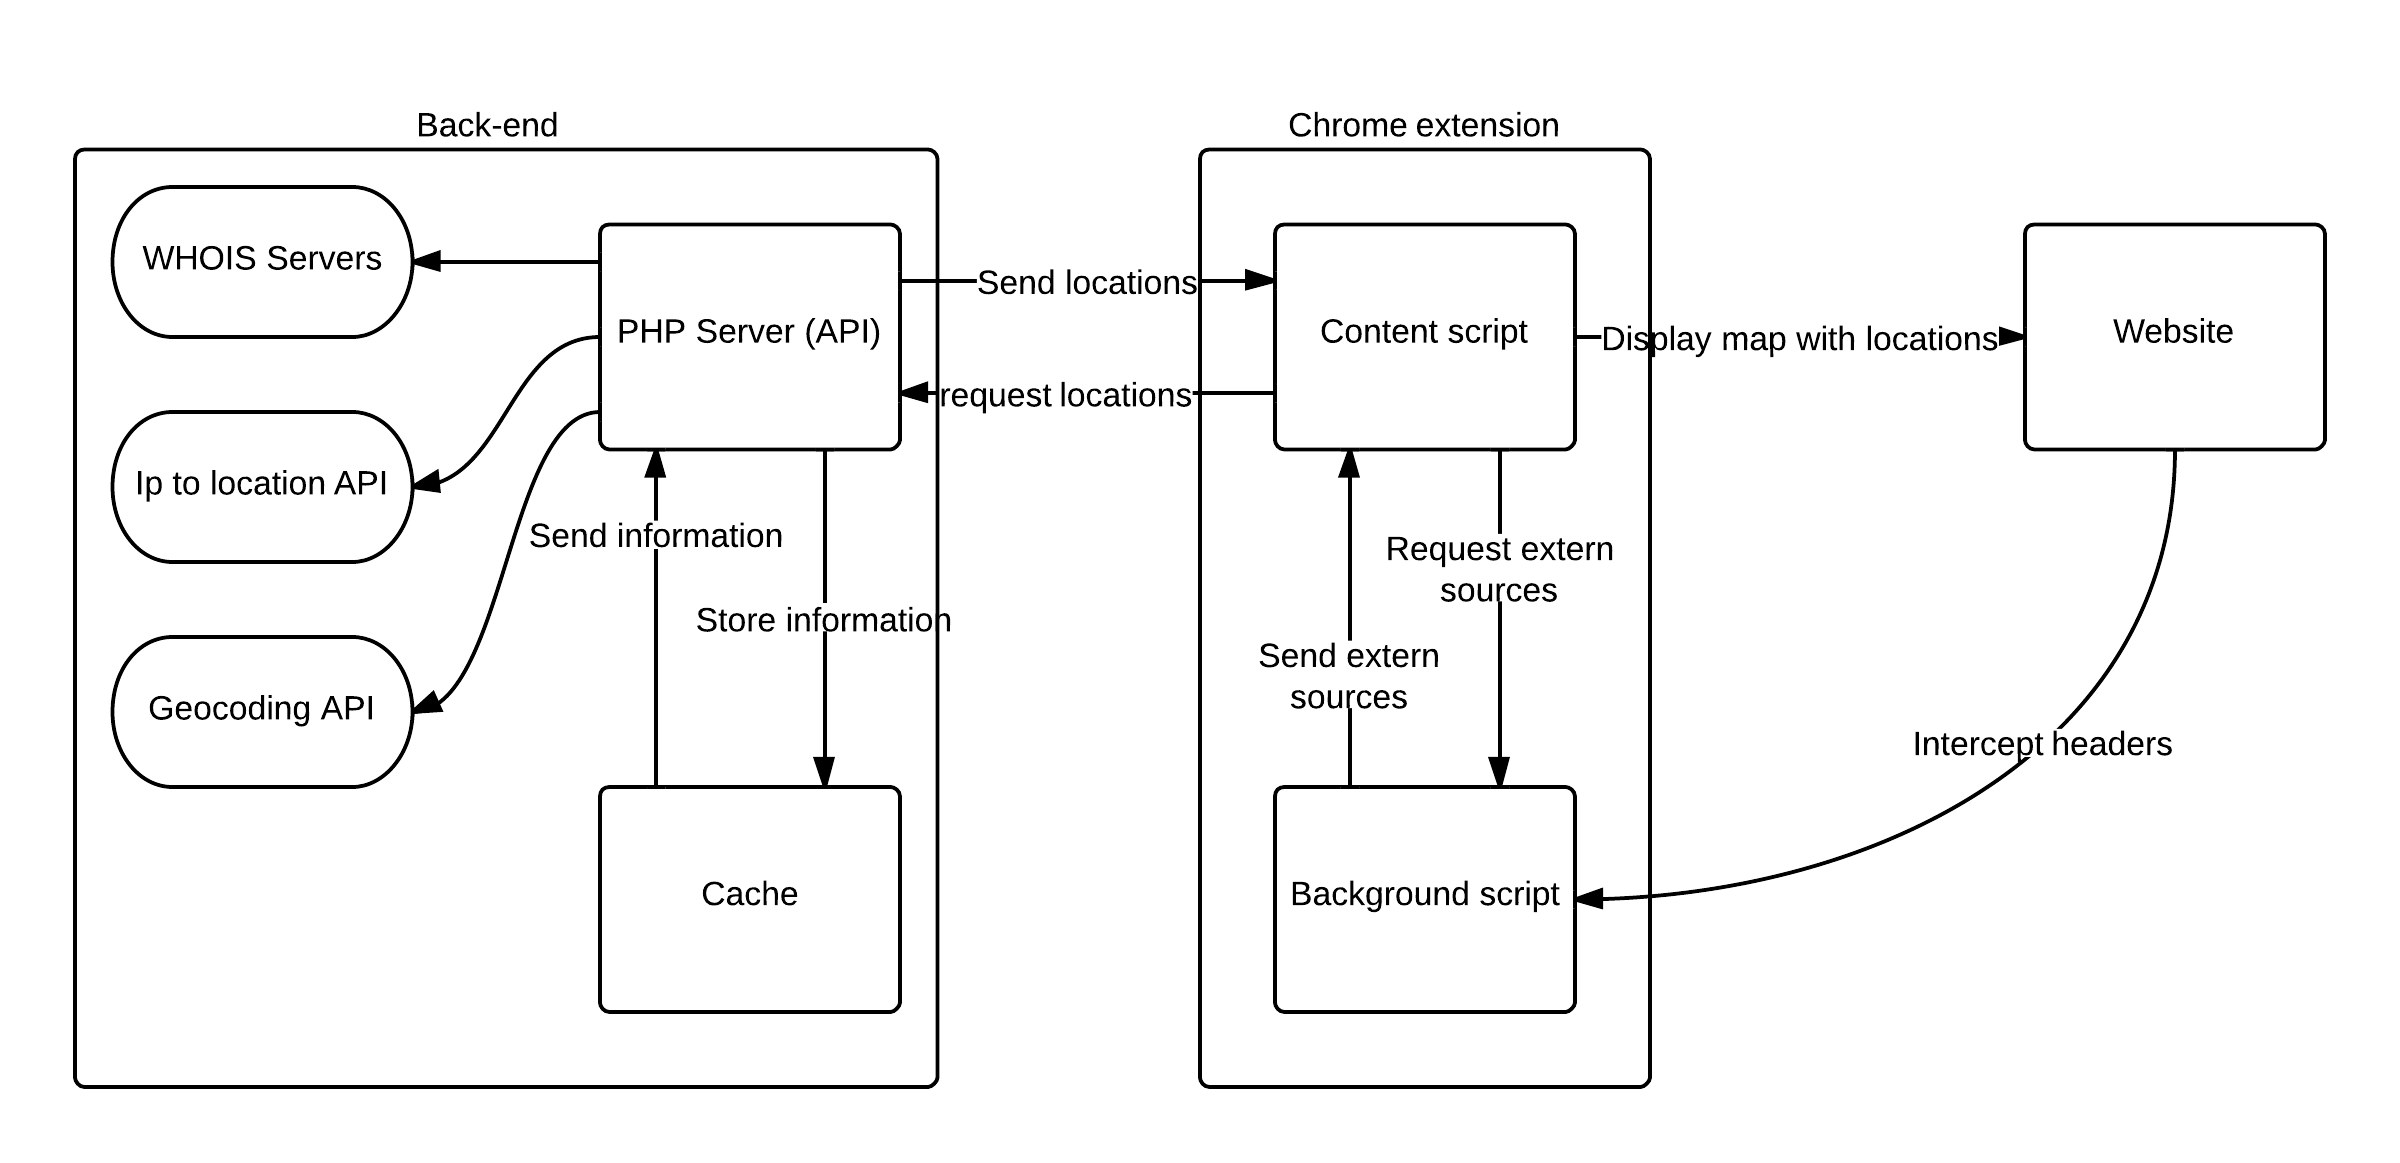
\includegraphics[width=1.2\textwidth, center]{img/implementation.png}
    \caption{Overview of the components of the back and front-end}
    \label{fig:implementation}
\end{figure}

\FloatBarrier

\section{Back-end}
The back-end is part of a program or tool which is invisible to the user. The interaction with users are handled indirectly via the graphical user interface (front-end). In this tool the back-end is a server which can collect all the necessary information for the locations of a website. Next the server is setup as an API. Other tools (front-end) or users can send a request to the API and it then returns the corresponding information.

\subsection{Server}
All the information about the geolocations is gathered en calculated by a server. The server uses PHP as the server-side script to collect the information. The specifications and installation manual of the server can be found in appendix A. The server needs classes for all the API's and services it needs to gather the geolocations.

\subsection{WHOIS Parser class}
One of the services that needs to be requested is WHOIS. The request is done with the \emph{fsockopen} function of PHP~\cite{php1}, which initiates a socket connection to the resource specified by the domain name.\\

As said before in the \emph{WHOIS} section in chapter \emph{Methods for data collection}, the format of the response of the WHOIS servers is very inconsistent.\\

To extract the correct information from the WHOIS response, the server needs to implement a WHOIS parser for each WHOIS server. Each TLD has its own WHOIS servers. Parsers for the following TLD's are implemented at the moment: "com", "net", "info", "org", "nl". Parse functions for other TLD's can be easily added to the code. There is a special parser for IP-adresses, which extracts the name and location of the host company of the resource specified by the IP-address.  \\

The parser also automatically follows the WHOIS registry referral chains until it finds the correct WHOIS registrars for the most complete WHOIS data. After requesting the information and parsing it, the WHOIS class returns the name and location of the registrant and registrar of the domain name, provided that that information is available.\\

(file: \emph{classes/whois.class.php})

\subsection{IP to location class}
To return the location of a resource or user identified by an IP-address, the server has a class that communicates with the IP-API Geolocation service~\cite{ipapi}. This API is free to use and is quite fast. PHP supports libcurl. This library can connect and communicate to many different types of servers with many different types of protocols~\cite{php2}. The class uses cURL functions to make a request to the IP-API. Unlike the WHOIS service, the response of this API is already formatted in serialized PHP and does not need to be parsed. \\

(file: \emph{classes/ip2loc.class.php})

\subsection{SSL Chain class}
To get the SSL certificate chain of a website that uses the https protocol, the server has a class that can make a request to a website with cURL (see previous section). The class sends some headers along with the request. Those headers tell cURL to verify the SSL certificates of the website. cURL then returns the certificates to the server. Just like the WHOIS response, the certificates are raw text, so they need to be parsed in order to find the name and location of the corresponding certification authorities. \\

(file: \emph{classes/sslchain.class.php})

\subsection{Google Geocoding API class}
This class implements the communication with the Google Geocoding API~\cite{google1}. Again, cURL is used to make a request to the API and return the response to the server. Besides the geolocation of an address, the API also returns a clean address and the bounding box of the area where the address resides. This bounding box is later used to calculate the radius of a geolocation. \\

(file: \emph{classes/geolocation.class.php})

\subsection{Caching}
Since all of the above API's and services have a request limit, a cache is implemented to reduce the number of request for each API. Each time a user makes a request to a service or API, its response is stored in SQLite database~\cite{sqlite}. SQLite is an embedded SQL database engine. Unlike most other SQL databases, SQLite does not have a separate server process. The whole database is stored in a single file. This makes SQLite small and fast. The SQLite library is available in PHP.\\

The requests and the responses are stored in the database together with a timestamp. This timestamp is used to check how long an entry is stored in the database. If the server wants to make a request to an API, it first checks in the cache if there is an entry with the same request. If that entry is not older than a certain time (for example 24 hours), the response stored alongside that request in the database is returned. This way the cache reduces the number of requests sent to the API's. \\

(file: \emph{getLocations.php} and \emph{db/cache.db})

\subsection{Setup server as Location API}
If the server has gathered and calculated all necessary information, that information needs to be made available for users or other tools. Therefore, the server acts as an API. Other resources can make requests to the server. In that request needs to be the domain name of the website from which the information is needed, which information to retrieve and in which format the information should be returned by the API. The current output formats are JSON, printed as an array and serialized PHP. \\

(file: \emph{index.php}) \\

In order to let the API know which information it needs to return, the request can be made with a fields code. There are 1024 different combinations possible for the fields. So the field code goes from 0 to 1023. When the server receives this field code, it gets converted to a binary value. Each bit of this binary value is either one or zero, where one means that the field needs to be collected and returned. To know which decimal value corresponds to which fields, there is a tool that generates the right code for the selected fields. The tool can be found on the documentation page of the API. See figure \ref{fig:field_generator} for a screenshot. \\

(file: \emph{pages/fields\_generator.html})

\begin{figure}[h!]
    \centering
    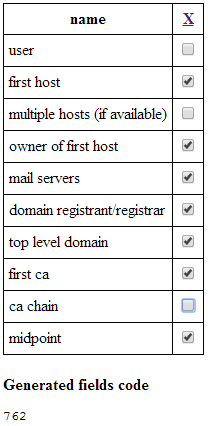
\includegraphics[width=0.35\textwidth, center]{img/code_generator.png}
    \caption{Fields code generator tool}
    \label{fig:field_generator}
\end{figure}

\FloatBarrier
\section{Front end}
The front end is an interface between the back end and the user. The front end can send request to the back end and visualize the response of the back end.

\subsection{Chrome extension}
In this implementation the front end is developed as a chrome extension. A chrome extension is a software program that modifies and enhances the functionality of the Chrome browser~\cite{google3}. Because the Chrome browser has the biggest market share worldwide, almost 50\% as of May 2014 according to StatCounter~\cite{stats}, the chrome extension is a good way to make the tool available for a lot of users. See figure \ref{fig:market_share1} and figure \ref{fig:market_share2} for a market share graph and a world map with the biggest browsers for each country~\cite{stats}. Because the back-end is setup as a general API, this extension could easily be ported to other browsers, like a FireFox extension.

\begin{figure}[h!]
    \centering
    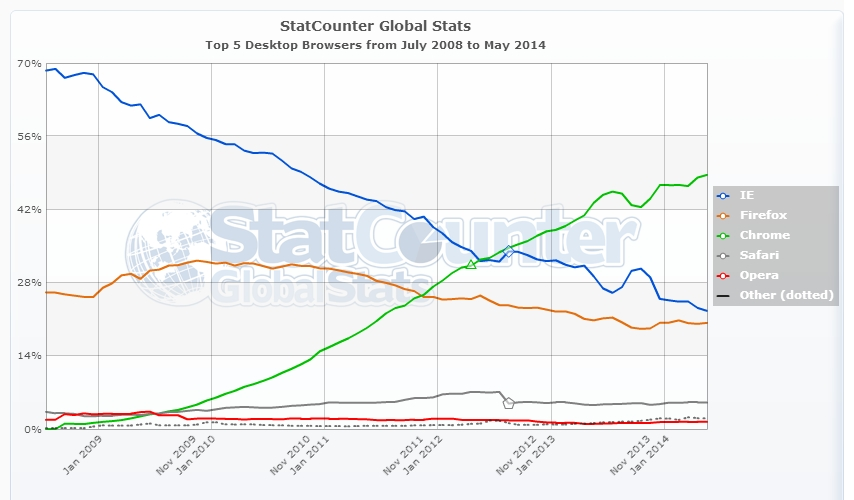
\includegraphics[width=1.0\textwidth, center]{img/market_share1.jpg}
    \caption{Browsers market share worldwide graph}
    \label{fig:market_share1}
\end{figure}

\begin{figure}[h!]
    \centering
    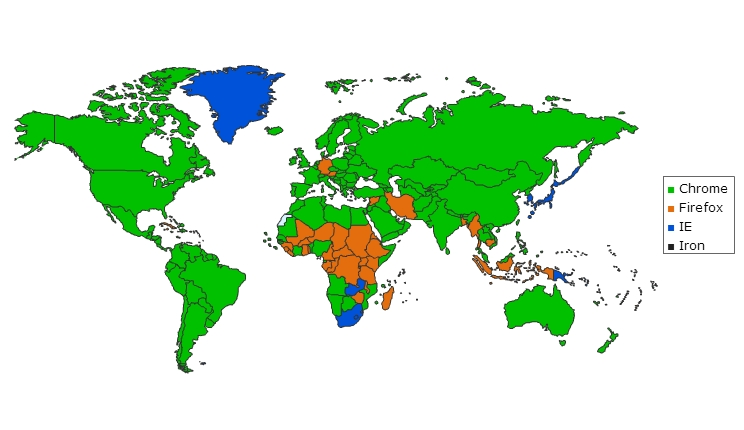
\includegraphics[width=1.0\textwidth, center]{img/market_share2.jpg}
    \caption{Browsers market share worldwide map}
    \label{fig:market_share2}
\end{figure}

\FloatBarrier

\begin{figure}[h!]
    \centering
    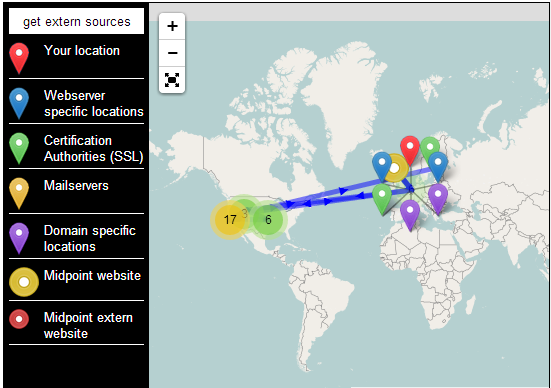
\includegraphics[width=1.0\textwidth, center]{img/tool.PNG}
    \caption{End result of the chrome extension}
    \label{fig:server}
\end{figure}

\subsection{Communication with server}
The chrome extension can send a request to the API of the back-end. The server will then handle the request and collect all necessary information. Because the chrome extension is built with JavaScript, the best output format is the JSON format. JavaScript can then parse and convert the JSON to JavaScript Objects.

\subsection{Content scripts}
The chrome extension adds a new JavaScript file to each website the user visits. This script handles the communication with the back-end for each website and also handles the visualization of the data received from the back-end. See the section \emph{Leaflet} for more information about the visualization.\\

(file: \emph{background.js})

\subsection{Retrieving external sources}
Besides the content scripts, the chrome extension also uses a background script for the whole browser session to capture and analyze the headers send by all open tabs in the Chrome browser. This script uses the Chrome webRequest API to analyze requests in-flight~\cite{google2}. The websites send requests for each external source they use. This also captures all external scripts and external content in frames. See chapter \emph{Methods for data collection}, section \emph{Intercepting headers} for more information about external sources and headers.\\

It is possible that requests for external sources are sent before the content script is loaded and able to receive the intercepted requests from the background script. Therefore, the background script stores all requests in a queue and also stores the tab id of the tab that made the request. If the content script is done loading and ready to receive the external sources from the background script it sends a request to the background script. The background script then returns all external sources belonging to the content script that made the request. When the content script has received all the external sources from the background script, it sends a message back as reply, so that the background script knows the content script has successfully received the information.\\

Because Chrome caches some requests, the background script might not find all headers if the script is trying to intercept them after Chrome has checked the cache. If a request is already in the cache, Chrome intercepts the request and retrieves the data from the cache. Thus the background script has to intercept the request before Chrome checks the cache. In figure \ref{fig:headers} all the states of a request in the Chrome browser are listed~\cite{google2}. In order to get all request, the background script has to intercept the headers at the \emph{onBeforeSendHeaders} state.\\

(file: \emph{external\_sources.js})

\begin{figure}[h!]
    \centering
    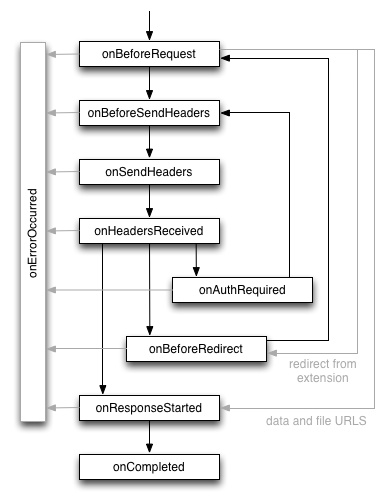
\includegraphics[width=0.5\textwidth, center]{img/headers.png}
    \caption{The event life cycle for successful requests}
    \label{fig:headers}
\end{figure}

\FloatBarrier
\section{Leaflet}
To display the world map with the different locations on each webpage, an open-source JavaScript library for mobile-friendly interactive maps, Leaflet~\cite{leaflet}, is implemented in the chrome extension. Besides that the library is very lightweight, it can be extended with a huge amount of plugins. With this library implemented, the content script can display a world map on the webpage and draw markers on that map.

\subsection{Markers}
After requesting the back-ends API to return the locations of the all the components of the website, these location are drawn onto the map as a marker. These markers can have different colors in order to distinguish the different components or groups of components. The tree structure of the locations is visualized by the arrowed lines between the markers. See figure \ref{fig:markers} for an example.

\begin{figure}[h!]
    \centering
    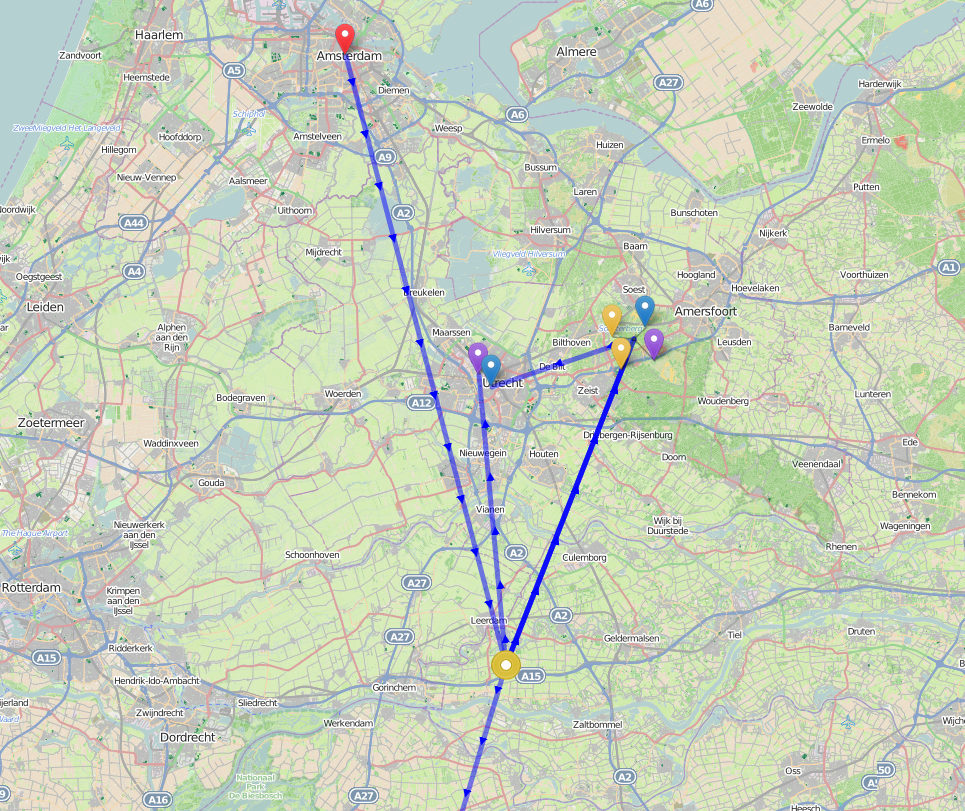
\includegraphics[width=0.75\textwidth, center]{img/markers.png}
    \caption{Markers with different colors on world map}
    \label{fig:markers}
\end{figure}

\FloatBarrier
\subsection{Precision}
In order to show the precision of a location to the user, circles with the same radius as the radius of the bounding box of the location are drawn around the marker. Figure \ref{fig:radius} shows an example of such a circle for a location with city-precision (Amsterdam). See section \emph{Precision of location} for more information about the precision and radius.

\begin{figure}[h!]
    \centering
    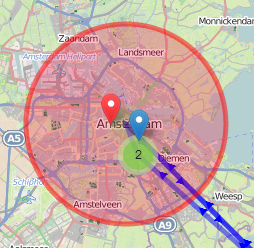
\includegraphics[width=0.4\textwidth, center]{img/radius.png}
    \caption{Marker with a circle to show the precision of the location}
    \label{fig:radius}
\end{figure}

\FloatBarrier
\subsection{Detailed information}
To see more detailed information about the locations, users can click on the markers and a popup will appear with information about that location. An example can be found in figure \ref{fig:popup}.

\begin{figure}[h!]
    \centering
    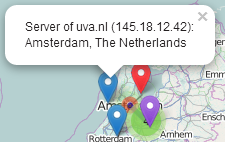
\includegraphics[width=0.4\textwidth, center]{img/popup.PNG}
    \caption{Marker with a popup to show more detailed information}
    \label{fig:popup}
\end{figure}

\FloatBarrier
\subsection{Clustering of markers}
The position of the locations may overlap each other on the world map. This means that markers are placed on top of each other, resulting in a cluttered view of the map. To overcome this problem, the Leaflet library is extended with a marker cluster plugin~\cite{leaflet2}. This plugin clusters the markers together if they overlap too much. An example of this clustering can be found in figure \ref{fig:cluster}.

\begin{figure}[h!]
    \centering
    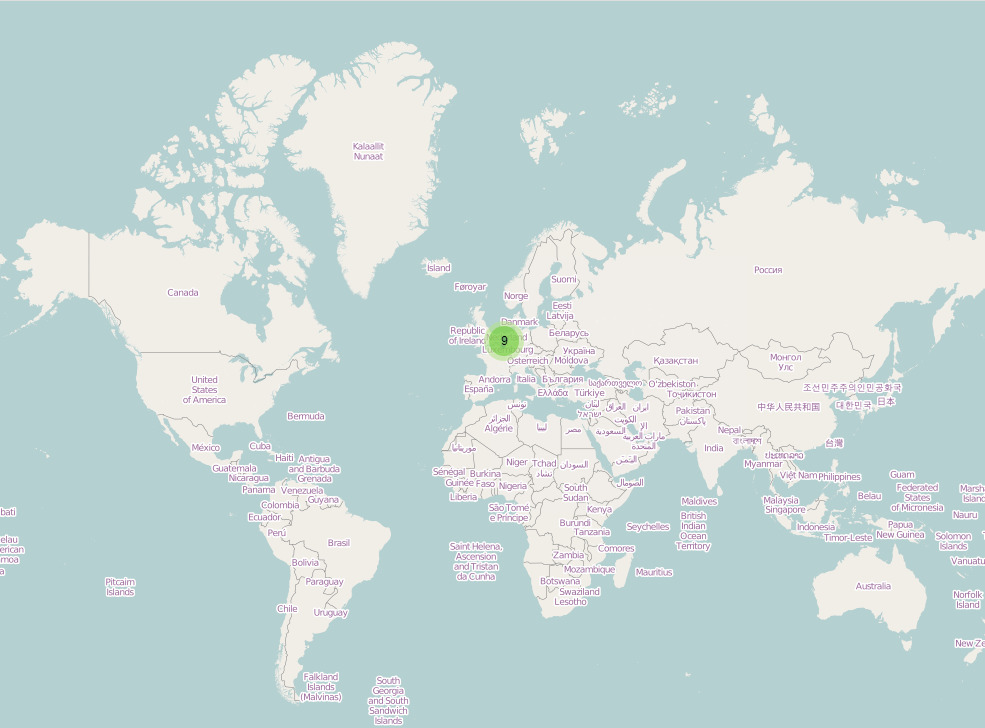
\includegraphics[width=1.0\textwidth, center]{img/cluster2.PNG}
    \caption{Markers clustered together}
    \label{fig:cluster}
\end{figure}

\begin{figure}[h!]
    \centering
    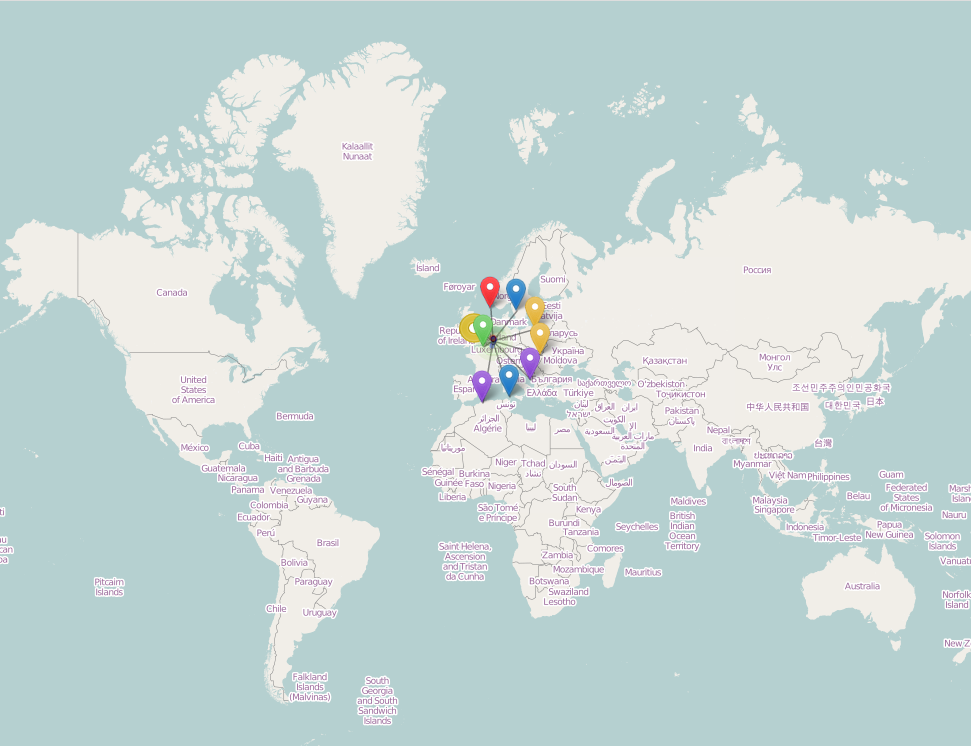
\includegraphics[width=1.0\textwidth, center]{img/cluster_open.PNG}
    \caption{Markers visible after user clicked on cluster}
    \label{fig:cluster_open}
\end{figure}

\FloatBarrier
\subsection{Displaying external sources}
To visualize the locations of the components of the external sources, the user can click on a button next to the map. This will send all received external sources from the background script to the back-end API and their locations will be displayed on the map.

\begin{figure}[h!]
    \centering
    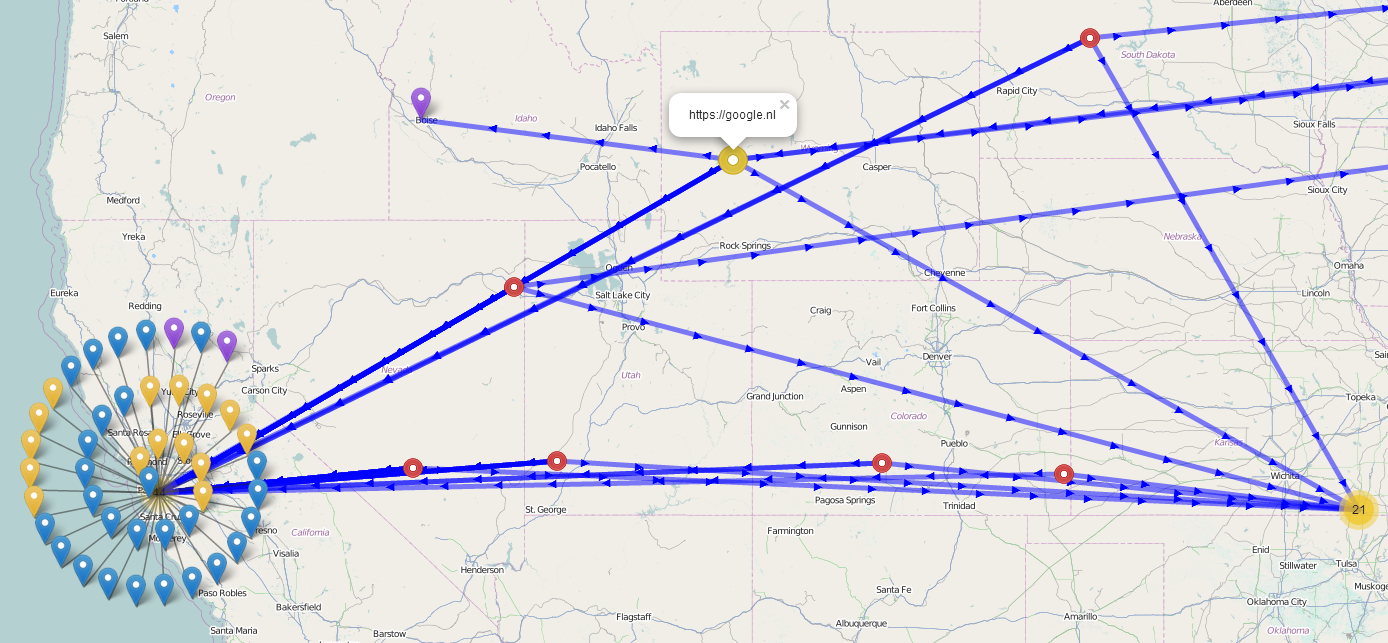
\includegraphics[width=1.0\textwidth, center]{img/google.PNG}
    \caption{Part of map of google.nl with external sources}
    \label{fig:google}
\end{figure}

\FloatBarrier
\chapter{Experiment}
To know whether the tool actually enables the users to say something about the trustworthiness of websites and to what extent that classification is better than without the tool, an user research needs to be done to determine the effectiveness of the tool in its current form. This chapter explains the setup of such an experiment and works out the results of this experiment.

\section{Setup}
In order to know how good a user can classify websites, a dataset of websites is needed with their correct classification acquainted. This research uses a set of 16 websites. 8 malicious websites and 8 'normal' websites. The normal websites are randomly selected from the web. So these websites can come from anywhere in the world. To verify the trustworthiness of these websites, extensive research is done to these sites. The contact details are checked, checked if they are not on any blacklist etc. To collect the 8 malicious websites, various blacklists~\cite{malwareblacklist, phishtank, wot} are used to collect a variety of malicious sites. The different types of malignancy in these 8 sites are malware, phising, exploit kit, spyware and Trojan.\\

To find out the effectiviness of the tool, the classification of the participants with use of the tool must be compared with the classification of the participants without the tool. To be able to compare these two, the participants first get to see all the websites in random order without the tool. Then the participants have to indicate for each website whether they trust the site or not. They can also indicate that they don't know if they can trust the site or not. \\ 

After the classification without the tool, the participants get to see the same websites again, but this time the tool is included with information about the locations of that website. Again the participants classify all websites or they indicate that they do not know it. All this data is stored in a database.

\begin{figure}[h!]
    \centering
    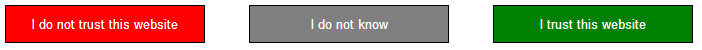
\includegraphics[width=0.9\textwidth, center]{img/options.PNG}
    \caption{Different options the participants could choose for each website}
    \label{fig:options}
\end{figure}

\FloatBarrier
\section{Results}
The raw data in the database needs to be analysed and worked out. The raw data can be found in the appendix B. The data of the malicious websites and the data of the normal websites are analysed separately, because their results may differ. 32 people participated in this experiment. Most of these people have an age between 20 and 30 years and are following university education. The ratio male/female is about one to one.\\

\subsection{Malicious websites}
In figure \ref{fig:tabel_bad} the results of the number of correct classified malicious website with and without the tool for each participant is shown.

\begin{figure}[h!]
    \centering
    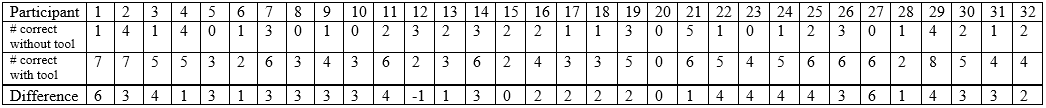
\includegraphics[width=1.2\textwidth, center]{img/tabel_bad.PNG}
    \caption{Number of correct classification of 8 malicious websites}
    \label{fig:tabel_bad}
\end{figure}

From this table we can calculate the mean percentages of correct classified malicious websites with and without the tool. Without the tool the participants had an average correct classified malicious websites of $1.75/8 * 100 \approx 21.9 \%$. With the tool that percentage was $4.38/8 *100 \approx 54.8 \%$.\\

To find out whether this difference of $32.9 \%$ is significant, a Paired samples t-tests can be done to find out whether two sets of data are significantly different from each other. Paired samples consist of a sample of matched pairs or one group of participants that has been tested twice.\\

The basic idea of a t-test is that in order to determine if from a normal distribution with standard deviation $σ$ the expected value $μ$ has a certain value $μ_0$, a sample from size $n$ is taken from that distribution en the sample average $\bar{X}$ is calculated. This average is following the normal distribution with expectation $μ_0$ and standarddeviation $σ/√n$ under the null hypothesis.

$$Z=\frac{\bar{X}-\mu_0}{\sigma/\sqrt{N}}$$

In this experiment the standard deviation is not known, thus the standard deviation is estimated by calculating the sample standard deviation $s$.

$$s = \sqrt{\frac{1}{N-1} \sum_{i=1}^N (x_i - \overline{x})^2}$$

However, T now follows the T-distribution under the null hypothesis instead of the normal distribution.

$$T=\frac{\bar{X}-\mu_0}{s/\sqrt{N}}$$

First calculate the sample standard deviation for the difference row in table \ref{fig:tabel_bad} where $N = 32$ and $\overline{x} = 2,625$:

$$s = \sqrt{\frac{1}{32-1} \sum_{i=1}^32 (x_i - 2,625)^2} \approx 1.60$$

If the tool does not have any effect on the effectiviness of the classification of malicious websites, the expectation $\mu_0$ is 0. Now $T$ can be calculated:

$$T=\frac{\bar{X}}{s/\sqrt{N}} = \frac{2.625}{1.60/\sqrt{32}} \approx 9.273$$

From a table of the t-distribution with $N - 1 = 31$ degrees of freedom can found that the p-value of this $T$ is smaller than 0.001\%:

$$ P(T(31) \ge 9{,}273) < 0.00001 $$

So the null hypothesis is rejected (considering the 5\% level) and thus the difference of 32.9\% is significant. An overview of these results can be found in figure \ref{fig:tabel_bad_results}

\begin{figure}[h!]
    \centering
    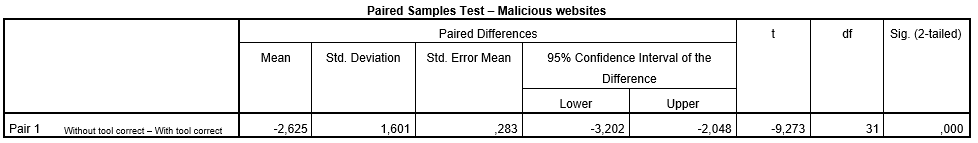
\includegraphics[width=1.2\textwidth, center]{img/tabel_bad_results.PNG}
    \caption{Results of paired samples t-test for malicious websites}
    \label{fig:tabel_bad_results}
\end{figure}


\FloatBarrier
\subsection{Normal websites}
In figure \ref{fig:tabel_good} the results of the number of correct classified malicious website with and without the tool for each participant is shown.\\

\begin{figure}[h!]
    \centering
    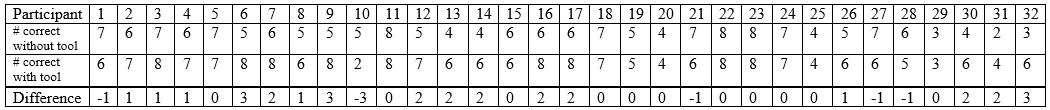
\includegraphics[width=1.2\textwidth, center]{img/tabel_good.PNG}
    \caption{Number of correct classification of 8 normal websites}
    \label{fig:tabel_good}
\end{figure}

Without the tool the participants had an average correct classified normal websites of $ 69.5 \%$. With the tool that percentage was $ 78.5 \%$.\\

To find out whether this difference of $9.0 \%$ is significant, the same calculation can be applied to the data of the normal websites. This time, the calculation steps are left out, because they are basically the same as the calculations for the malicious websites, only with different data. The results can be found in figure \ref{fig:tabel_good_results}.

\begin{figure}[h!]
    \centering
    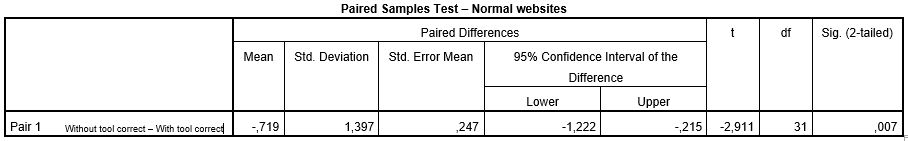
\includegraphics[width=1.2\textwidth, center]{img/tabel_good_results.PNG}
    \caption{Results of paired samples t-test for normal websites}
    \label{fig:tabel_good_results}
\end{figure}

From the table with the results can be read that the p-value is 0.007:

$$ P(T(31) \ge 2{,}911) < 0.01 $$

So the null hypothesis is again rejected (considering the 5\% level) and thus the difference of 9.0\% is significant.

\subsection{Certainty}
As the participants also had the possibility to choose the "Don't know" option, the certainties of the classifications with the tool and without the tool can also be compared to each other. This can be done for both types of websites, the normal websites and the malicious websites.\\

For normal websites the certainty increased from 84.0\% to 90.2\% and for malicious websites the certainty increased from 82.4\% to 87.1\%. To check whether these increases are significant, again the paired sample t-test can be executed. The calculation are the same as the calculation steps in previous two t-tests, so only the results are shown in figure \ref{fig:zekerheid}

\begin{figure}[h!]
    \centering
    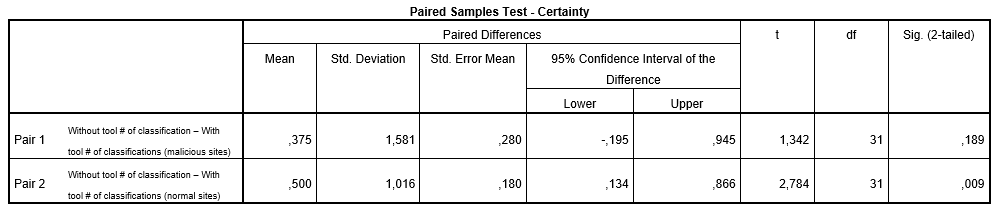
\includegraphics[width=1.2\textwidth, center]{img/zekerheid.PNG}
    \caption{Results of paired samples t-tests for certainty of the classification of normal websites and malicious websites}
    \label{fig:zekerheid}
\end{figure}

The results show that the increase for the normal websites is indeed significant with a p-value of 0.009, but the increase for malicious websites is not significant with a p-value of 0.189 (considering the 5\% level).

\FloatBarrier
\chapter{In conclusion}
\section{Discusion}
The results of the experiment are very promising. Both the classification of malicious websites and normal websites improved significantly with the tool. The certainty of the classifications also increased when the users were using the tool. However, users still have to classify the websites manually and put effort in classifying websites. Even with the tool it can still be hard for a user to classify a website as malicious or not.

\subsection{Future work}
Ideally, the user should be notified automatically when he is visiting a malicious website, without putting any of his own effort into the classification. In future research Machine learning could be considered to achieve this goal. With Machine learning the tool itself could learn certain suspicious patterns in the geographic features of websites. When the tool detects a suspicious pattern, it can alert the user that the site he wants to visit might be malicious.\\

In the \emph{Related work} section a few other studies are mentioned that use Machine learning to automatically classify websites using certain features (URL-based features or content-based features). However, these studies all lack geographical features. The combination of the features of these studies with the geographical features of this thesis could, with the help of Machine learning, give a good evaluation about the trustworthiness of websites.

\subsection{Privacy}
As the tool could potentially keep track of the browsing history of a user, this could give some good insight in the patterns of locations of the websites the user visits. This also raises some privacy issues. The browsing patterns of a user could be abused by malevolent people or companies. To avoid this privacy issue, users have the ability to run their own server where the privacy-sensitive information is stored. This also alleviates the problem of the limitations set by the different services and API's used. The requirements and the setup of an own server can be found in Appendix A.

\begin{figure}[h!]
    \centering
    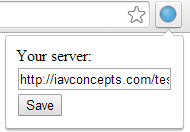
\includegraphics[width=0.3\textwidth, center]{img/server.PNG}
    \caption{Ability to run own server with chrome extension}
    \label{fig:server}
\end{figure}

\FloatBarrier
\section{Conclusion}
The geographical locations of website is a feature that is not yet used in the classification of websites, but shows promising results for the future. This thesis looked if the geographical features of websites could help the user to evaluate the trustworthiness of websites. To achieve this, first there must be examined which components may have a location and how those locations can be retrieved. Different API's and services and own calculation combined resulted in an API, which can retrieve all the necessary information. Subsequently, this thesis looked at the strategies for the presentation of the retrieved information and good ways to combine that information. All this knowledge is then combined in a tool for the user which might help him classify websites. \\

The experiment where the participants had to classify websites with and without the tool showed that the tool in its current form improved the classification of both malicious and normal websites significally and also improved the certainty of the classifications. When the geographical features found in this thesis are combined with features from related research, a technique might be developed that automatically evaluates websites that is better than current approaches.\\

All in all, this thesis has successfully proved that geographical features can play an important role in determining the trustworthiness of websites. By looking at the geographical consistency of a website, a good prediction can be made about the trustworthiness of that website. Hopefully this knowledge will be used in the future in other research with the ultimate goal to have users prevail in their stride against malicious websites.

\printbibliography

\appendix
\chapter{Setup server and chrome extension manual and requirements}
\section{Server requirements}
\begin{itemize}
\item A webserver that supports PHP, such as Apache (Linux) or IIS (Windows)
\item A webserver with at least 1 megabyte of available disk space.
\item PHP 5.3.2+
\item SQLite extension for PHP
\end{itemize}
\section{Server setup}
Download the server files from https://github.com/laurensV/TrustingWebsites/tree/master/server and put them on your webserver.

\section{Chrome extension setup}
\begin{itemize}
\item Download the extension files from https://github.com/laurensV/TrustingWebsites/tree/master/chrome-extension.
\item Open Google Chrome browser and navigate to \emph{extra > extension}.
\item check the checkbox next to "developer mode" and choose [Load extracted extension]
\item Locate the previously downloaded extension files and enable the extension.
\item click on the icon of the extension and fill in the domain name or ip-address of your server.
\end{itemize}
\chapter{Raw data experiment}
-1  =  I do not trust this website\\
 0  =  I do not know\\
 1  =  I trust this website
 \begin{table}[h!]
\parbox{.45\linewidth}{
\centering
\begin{tabular}{lllllllll}
\textbf{1}  & 1 & 1  & 1  & 1  & 0  & 0  & 1  & -1 \\
\textbf{2 } & 1 & 1  & 1  & 1  & -1 & -1 & -1 & -1 \\
\textbf{3 } & 1 & -1 & 1  & 1  & 0  & 1  & 1  & 1  \\
\textbf{4 } & 1 & -1 & 1  & 1  & 1  & -1 & -1 & -1 \\
\textbf{5 } & 1 & 1  & 0  & 1  & 1  & 1  & 1  & 1  \\
\textbf{6 } & 1 & 1  & -1 & 1  & 1  & 1  & 1  & 0  \\
\textbf{7 } & 1 & 1  & 1  & -1 & 0  & -1 & -1 & 1  \\
\textbf{8 } & 0 & 1  & 1  & 1  & 0  & 1  & 0  & 1  \\
\textbf{9 } & 1 & 1  & 1  & 1  & 0  & 1  & 0  & -1 \\
\textbf{10} & 1 & 1  & 0  & 0  & 0  & 1  & 1  & 1  \\
\textbf{11} & 1 & 1  & -1 & 1  & 1  & 1  & 1  & -1 \\
\textbf{12} & 1 & 1  & 1  & 1  & 1  & -1 & -1 & -1 \\
\textbf{13} & 0 & 1  & -1 & 1  & 1  & -1 & 1  & 1  \\
\textbf{14} & 0 & 1  & 0  & -1 & -1 & 0  & 0  & -1 \\
\textbf{15} & 1 & 1  & 0  & 1  & -1 & 0  & -1 & 1  \\
\textbf{16} & 1 & 1  & 1  & 1  & 1  & -1 & -1 & 1  \\
\textbf{17} & 1 & 1  & -1 & 1  & 1  & 1  & 1  & 1  \\
\textbf{18} & 1 & 1  & 1  & 1  & 1  & 1  & -1 & 1  \\
\textbf{19} & 0 & 1  & -1 & -1 & 1  & 1  & -1 & 1  \\
\textbf{20} & 1 & 1  & 1  & 0  & 0  & 0  & 0  & 1  \\
\textbf{21} & 1 & 1  & -1 & -1 & -1 & -1 & -1 & 1  \\
\textbf{22} & 1 & 1  & -1 & 1  & 1  & 1  & 1  & 1  \\
\textbf{23} & 1 & 1  & 0  & 1  & 1  & 1  & 1  & 0  \\
\textbf{24} & 1 & 1  & 0  & 1  & 1  & -1 & 0  & 1  \\
\textbf{25} & 1 & 1  & 1  & 1  & -1 & 0  & -1 & 1  \\
\textbf{26} & 1 & 1  & -1 & 1  & 0  & -1 & -1 & 1  \\
\textbf{27} & 1 & 1  & 1  & 0  & 0  & 1  & 1  & 1  \\
\textbf{28} & 1 & 0  & 1  & 1  & 1  & -1 & 1  & 1  \\
\textbf{29} & 1 & 1  & -1 & -1 & 0  & -1 & -1 & 1  \\
\textbf{30} & 1 & 1  & -1 & 1  & 0  & 0  & -1 & 1  \\
\textbf{31} & 0 & 1  & 0  & 1  & 0  & 0  & 0  & -1 \\
\textbf{32} & 1 & 1  & -1 & -1 & 0  & 1  & 0  & 1 
\end{tabular}
\caption{Results without tool malicious websites}
}
\parbox{.45\linewidth}{
\centering
\begin{tabular}{lllllllll}
\textbf{1}  & -1 & -1 & -1 & 0  & -1 & -1 & -1 & -1 \\
\textbf{2}  & -1 & -1 & 1  & -1 & -1 & -1 & -1 & -1 \\
\textbf{3}  & 1  & -1 & -1 & -1 & 1  & 1  & -1 & -1 \\
\textbf{4}  & 1  & -1 & 1  & -1 & -1 & 1  & -1 & -1 \\
\textbf{5}  & 1  & 0  & -1 & -1 & 1  & 1  & -1 & 1  \\
\textbf{6}  & -1 & 0  & 1  & 1  & 0  & 1  & -1 & 1  \\
\textbf{7}  & -1 & 1  & 1  & -1 & -1 & -1 & -1 & -1 \\
\textbf{8}  & 0  & 0  & -1 & -1 & 0  & 0  & 0  & -1 \\
\textbf{9}  & 1  & -1 & 1  & -1 & 1  & 1  & -1 & -1 \\
\textbf{10} & 0  & 1  & -1 & -1 & -1 & 1  & 1  & 1  \\
\textbf{11} & -1 & -1 & -1 & -1 & 1  & 1  & -1 & -1 \\
\textbf{12} & -1 & -1 & 1  & 1  & 1  & 1  & 1  & 1  \\
\textbf{13} & -1 & 1  & 1  & -1 & 0  & 1  & -1 & 1  \\
\textbf{14} & 1  & -1 & -1 & -1 & -1 & 1  & -1 & -1 \\
\textbf{15} & 1  & 1  & 0  & 0  & -1 & 0  & -1 & 1  \\
\textbf{16} & -1 & -1 & 1  & 0  & 0  & 0  & -1 & -1 \\
\textbf{17} & 1  & 1  & 1  & -1 & -1 & 1  & -1 & 1  \\
\textbf{18} & 1  & -1 & -1 & -1 & 1  & 1  & 1  & 0  \\
\textbf{19} & 1  & -1 & -1 & -1 & -1 & 1  & -1 & 1  \\
\textbf{20} & 1  & 1  & 1  & 0  & 0  & 1  & 0  & 0  \\
\textbf{21} & -1 & -1 & -1 & -1 & -1 & 1  & -1 & 1  \\
\textbf{22} & 1  & -1 & -1 & -1 & -1 & 1  & 1  & -1 \\
\textbf{23} & 1  & 1  & -1 & -1 & -1 & 1  & 1  & -1 \\
\textbf{24} & -1 & 1  & -1 & -1 & 1  & -1 & -1 & 1  \\
\textbf{25} & -1 & -1 & 0  & -1 & -1 & -1 & -1 & 1  \\
\textbf{26} & 0  & -1 & -1 & -1 & -1 & 1  & -1 & -1 \\
\textbf{27} & 1  & -1 & -1 & -1 & -1 & 1  & -1 & -1 \\
\textbf{28} & 0  & -1 & 0  & 0  & 0  & 0  & 1  & -1 \\
\textbf{29} & -1 & -1 & -1 & -1 & -1 & -1 & -1 & -1 \\
\textbf{30} & -1 & -1 & 1  & -1 & -1 & 1  & -1 & 1  \\
\textbf{31} & -1 & -1 & 0  & 0  & 0  & -1 & 0  & -1 \\
\textbf{32} & 1  & 1  & -1 & -1 & -1 & 1  & -1 & 1 
\end{tabular}
\caption{Results with tool malicious websites}
}
\end{table}

 \begin{table}[h!]
\parbox{.45\linewidth}{
\centering
\begin{tabular}{lllllllll}
\textbf{1}  & 0  & 1  & 1  & 1  & 1  & 1  & 1  & 1 \\
\textbf{2 } & -1 & -1 & 1  & 1  & 1  & 1  & 1  & 1 \\
\textbf{3 } & 1  & -1 & 1  & 1  & 1  & 1  & 1  & 1 \\
\textbf{4 } & 0  & 1  & 1  & 1  & -1 & 1  & 1  & 1 \\
\textbf{5 } & 0  & 1  & 1  & 1  & 1  & 1  & 1  & 1 \\
\textbf{6 } & 0  & 1  & 0  & 0  & 1  & 1  & 1  & 1 \\
\textbf{7 } & 0  & -1 & 1  & 1  & 1  & 1  & 1  & 1 \\
\textbf{8 } & -1 & 0  & 0  & 1  & 1  & 1  & 1  & 1 \\
\textbf{9 } & 0  & 0  & 1  & 1  & 1  & 1  & -1 & 1 \\
\textbf{10} & 1  & 1  & 0  & 1  & 0  & 0  & 1  & 1 \\
\textbf{11} & 1  & 1  & 1  & 1  & 1  & 1  & 1  & 1 \\
\textbf{12} & 1  & -1 & -1 & 1  & 1  & -1 & 1  & 1 \\
\textbf{13} & -1 & -1 & 0  & 1  & 1  & 1  & 0  & 1 \\
\textbf{14} & -1 & 0  & -1 & 1  & 0  & 1  & 1  & 1 \\
\textbf{15} & 0  & 1  & 0  & 1  & 1  & 1  & 1  & 1 \\
\textbf{16} & 0  & -1 & 1  & 1  & 1  & 1  & 1  & 1 \\
\textbf{17} & -1 & 1  & 1  & 1  & -1 & 1  & 1  & 1 \\
\textbf{18} & 1  & -1 & 1  & 1  & 1  & 1  & 1  & 1 \\
\textbf{19} & -1 & 1  & -1 & 1  & 0  & 1  & 1  & 1 \\
\textbf{20} & 0  & 0  & 0  & 1  & 0  & 1  & 1  & 1 \\
\textbf{21} & -1 & 1  & 1  & 1  & 1  & 1  & 1  & 1 \\
\textbf{22} & 1  & 1  & 1  & 1  & 1  & 1  & 1  & 1 \\
\textbf{23} & 1  & 1  & 1  & 1  & 1  & 1  & 1  & 1 \\
\textbf{24} & -1 & 1  & 1  & 1  & 1  & 1  & 1  & 1 \\
\textbf{25} & 0  & 0  & -1 & 1  & 1  & 0  & 1  & 1 \\
\textbf{26} & 0  & -1 & 1  & 1  & 1  & -1 & 1  & 1 \\
\textbf{27} & 1  & 1  & 0  & 1  & 1  & 1  & 1  & 1 \\
\textbf{28} & -1 & -1 & 1  & 1  & 1  & 1  & 1  & 1 \\
\textbf{29} & -1 & -1 & -1 & 1  & 1  & 0  & 0  & 1 \\
\textbf{30} & -1 & -1 & 0  & 1  & 1  & 1  & -1 & 1 \\
\textbf{31} & -1 & 0  & 0  & 0  & 1  & 0  & -1 & 1 \\
\textbf{32} & -1 & 0  & 0  & -1 & 0  & 1  & 1  & 1
\end{tabular}
\caption{Results without tool normal websites}
}
\parbox{.45\linewidth}{
\centering
\begin{tabular}{llllllllll}
\textbf{1}  & 1  & 1  & 1  & 1  & -1 & -1 & 1  & 1 \\
\textbf{2 } & -1 & 1  & 1  & 1  & 1  & 1  & 1  & 1 \\
\textbf{3 } & 1  & 1  & 1  & 1  & 1  & 1  & 1  & 1 \\
\textbf{4 } & 1  & 1  & 1  & 1  & -1 & 1  & 1  & 1 \\
\textbf{5 } & 1  & 1  & 0  & 1  & 1  & 1  & 1  & 1 \\
\textbf{6 } & 1  & 1  & 1  & 1  & 1  & 1  & 1  & 1 \\
\textbf{7 } & 1  & 1  & 1  & 1  & 1  & 1  & 1  & 1 \\
\textbf{8 } & 0  & 1  & 1  & 1  & 0  & 1  & 1  & 1 \\
\textbf{9 } & 1  & 1  & 1  & 1  & 1  & 1  & 1  & 1 \\
\textbf{10} & -1 & 0  & 0  & 1  & 0  & -1 & 0  & 1 \\
\textbf{11} & 1  & 1  & 1  & 1  & 1  & 1  & 1  & 1 \\
\textbf{12} & 1  & -1 & 1  & 1  & 1  & 1  & 1  & 1 \\
\textbf{13} & 1  & 1  & -1 & 1  & -1 & 1  & 1  & 1 \\
\textbf{14} & 1  & 1  & 1  & 1  & 0  & 1  & 1  & 0 \\
\textbf{15} & 1  & 1  & 0  & 1  & 0  & 1  & 1  & 1 \\
\textbf{16} & 1  & 1  & 1  & 1  & 1  & 1  & 1  & 1 \\
\textbf{17} & 1  & 1  & 1  & 1  & 1  & 1  & 1  & 1 \\
\textbf{18} & -1 & 1  & 1  & 1  & 1  & 1  & 1  & 1 \\
\textbf{19} & -1 & 1  & -1 & 1  & -1 & 1  & 1  & 1 \\
\textbf{20} & 0  & 0  & 0  & 1  & 0  & 1  & 1  & 1 \\
\textbf{21} & -1 & 1  & 1  & 1  & -1 & 1  & 1  & 1 \\
\textbf{22} & 1  & 1  & 1  & 1  & 1  & 1  & 1  & 1 \\
\textbf{23} & 1  & 1  & 1  & 1  & 1  & 1  & 1  & 1 \\
\textbf{24} & -1 & 1  & 1  & 1  & 1  & 1  & 1  & 1 \\
\textbf{25} & 0  & 0  & -1 & -1 & 1  & 1  & 1  & 1 \\
\textbf{26} & -1 & -1 & 1  & 1  & 1  & 1  & 1  & 1 \\
\textbf{27} & -1 & 1  & 1  & 1  & -1 & 1  & 1  & 1 \\
\textbf{28} & 0  & 0  & 1  & 1  & -1 & 1  & 1  & 1 \\
\textbf{29} & -1 & 1  & 0  & 1  & 0  & 0  & -1 & 1 \\
\textbf{30} & 1  & -1 & 1  & -1 & 1  & 1  & 1  & 1 \\
\textbf{31} & -1 & 0  & 1  & 0  & -1 & 1  & 1  & 1 \\
\textbf{32} & 0  & 1  & 1  & 1  & -1 & 1  & 1  & 1
\end{tabular}
\caption{Results with tool normal websites}
}
\end{table}




\end{document}